\documentclass[../../main]{subfiles}

\begin{document}
\chapter{数ベクトル空間}
\label{chapter:numerical_vector_space}

\section{イントロダクション}
\label{section:numerical_vector_space_introduction}

\cref{chapter:numerical_vector_space}では,数ベクトル空間\(\numset{K}^n\)(\(\numset{K}=\numset{R},\numset{C}\))に関する理論を扱う.
信号解析において,この理論は
\begin{enumerate}
  \item 離散時間信号の時系列分析
  \item 観測値をモデルに対応づける回帰・判別分析
\end{enumerate}
という,2つの方向に応用される.

音声信号処理は前者の主要な例である.音声信号を計算機で処理するには,時々刻々と値が変わる信号を有限長のデータで表現しなければならない.
たとえば,CDでは音声信号の瞬時値を1秒あたり44100個記録している.すなわち,時刻\(t\)秒における瞬時値を\(x(t)\),収録時間を\(T\)秒とおくと,CDには数列\(\seq{x(n/44100)}_{n=0}^{44100T-1}\)が記録されている.
そこで,収録されたデータを\(\numset{K}^{44100T}\)の元とみなせば,\(\numset{K}^n\)に関する理論に基づいて音声を解析できる.

後者の主要な例は最小2乗法である.実験で得られた標本を理論と見比べるとき,理論から得られる式へのあてはめ(回帰)がしばしば試される.
あてはまりのよさを示す指標はいろいろあるが,最もポピュラーなのは2乗誤差を指標にする最小2乗法である.本書ではこの最小2乗法を,内積と関連づけ幾何的に説明する.

\pagebreak

\section{直交射影}

本節では,あるベクトルを他のベクトルの線型結合で近似する手法を説明する.\cref{chapter:numerical_vector_space}において\(\numset{K}\)は\(\numset{R}\)か\(\numset{C}\)を意味し,
\(\innerp{\holder}{\holder}\)は\(\numset{K}^n\)の標準内積を意味する.また,\(\vnorm{\vect{x}}=\sqrt{\innerp{\vect{x}}{\vect{x}}}\)を\(\vect{x}\)の\termdef{ノルム}\index{のるむ@ノルム}\indexsymbol{\(\vnorm{\holder}\)}(norm)と呼ぶ.

\subsection{直交射影}

\begin{wrapfigure}[8]{o}{0pt}
  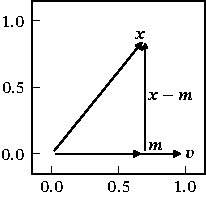
\includegraphics{figures/proj2d.pdf}
\end{wrapfigure}

\(\numset{K}^n\)のベクトル\(\vect{x}\),部分空間\(V\)が与えられたとき,\(V\)の元で\(\vect{x}\)に最も近いベクトル,すなわち,距離\(\vnorm{\vect{x}-\vect{m}}\)を最小にする\(\vect{m}\in V\)について考えよう.

\(\numset{K}^n\)が平面\(\numset{R}^2\)で,\(V\)があるベクトル\(\vect{v}\neq\zvec\)により生成される直線\(\spannedby\Set{\vect{v}}\)の場合,\(\vect{m}\)は図の位置にある.
図を見ると,\(\vect{x}-\vect{m}\)は\(\vect{v}\)と直交しているのが分かる.

一般の部分空間\(V\subseteq\numset{K}^n\)においても,直交性と最良近似には密接な関係がある.その証明へと入る前に,便利な記法を2つ定義しておく.

\begin{definition}{argmin,argmax}{argmin_argmax}\index{argmin@\(\argmin\)}\index{argmax@\(\argmax\)}
  集合\(S\)を定義域に含む実数値関数\(f\)に対して,集合\(\argmin_{x\in S}f(x)\),\(\argmax_{x\in S}f(x)\)を以下の通り定義する.
  \begin{gather*}
    \argmin_{x\in S}f(x) = \Set{x\in S\given\text{任意の\(y\in S\)に対して\(f(y)\geq f(x)\)}}, \\
    \argmax_{x\in S}f(x) = \Set{x\in S\given\text{任意の\(y\in S\)に対して\(f(y)\leq f(x)\)}}
  \end{gather*}
\end{definition}

\cref{definition:argmin_argmax}からただちに,次のことが分かる.

\begin{proposition}{}{}
  \(S\)の元\(a\)に関する以下の条件は同値であり,同様のことが\(\argmax\)についても成り立つ.
  \begin{enumerate}
    \item \(a\in\argmin_{x\in S}f(x)\)である.
    \item \(f(a)\)は集合\(\ran{f}{S}=\Set{f(x)\given x\in S}\)の最小元である.
  \end{enumerate}
\end{proposition}

\begin{wrapfigure}[8]{o}{0pt}
  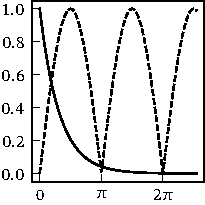
\includegraphics{figures/argmin.pdf}
\end{wrapfigure}

図は\(\napr^{-x}\)と\(\abs{\sin x}\)のグラフである.\(\napr^{-x}\to 0\)(\(x\to\infty\))であるが,\(\napr^{-x}=0\)となる実数\(x\)は存在しない.そのため\indexsymbol{\(\emptyset\)}
\begin{gather*}
  \argmin_{x\in\coival{0}{+\infty}}\napr^{-x} = \emptyset\quad\text{(空集合)}, \\
  \argmin_{x\in\coival{0}{+\infty}}\abs{\sin x} = \Set{0,\krez,2\krez,\dotsc}
\end{gather*}
である.このように,\(\argmin_{x\in S}f(x)\)は空になることも,無限集合になることもある.

\(\numset{K}=\numset{R}\)の場合も同様に証明できるので,\cref{proposition:finite_projection}まで証明では\(\numset{K}=\numset{C}\)を仮定する.また,部分空間が\(\Set{\zvec}\)でないことも仮定する.

\begin{lemma}{}{binomial_square}
  \(\vnorm{\vect{x}+\vect{y}}^2=\vnorm{\vect{x}}^2+2\rpart\innerp{\vect{x}}{\vect{y}}+\vnorm{\vect{y}}^2\)(\(\vect{x},\vect{y}\in\numset{K}^n\))である.
\end{lemma}

\begin{proof}
  \(\vnorm{\vect{x}+\vect{y}}^2=\innerp{\vect{x}+\vect{y}}{\vect{x}+\vect{y}}\)の右辺を展開すれば示せる.
\end{proof}

\begin{proposition}{}{finite_convex_projection}
  \(\vect{x}\in\numset{K}^n\)かつ,\(V\)は\(\numset{K}^n\)の部分空間とする.
  このとき,\(\argmin_{\vect{y}\in V}\vnorm{\vect{x}-\vect{y}}\)はただ一つの元からなる集合である.
\end{proposition}

\begin{proof}
  本証明に限り,\(\sum_{i=1}^m\)(\(m=\dim V\))を\(\sum\)と略記する.
  任意に\(\vect{y}\in V\)をとる.\(\basis{B}=\Set{\vect{e}_1,\dots,\vect{e}_m}\)を\(V\)の正規直交基底とすると,\(\vect{y}\)は\(\basis{B}\)の元の線型結合で\(\vect{y}=\sum z_i\vect{e}_i\)と書ける.
  また\(\innerp{\vect{e}_i}{\vect{e}_j}=\kdelta{i}{j}\)だから
  \[
    \vnorm*{\sum z_i\vect{e}_i}^2 = \innerp*{\sum_{i=1}^mz_i\vect{e}_i}{\sum_{j=1}^mz_j\vect{e}_j}
    = \sum_{i=1}^mz_i\sum_{j=1}^m\conj{z}_j\innerp{\vect{e}_i}{\vect{e}_j}
    = \sum z_i\conj{z}_i
    = \sum\abs{z_i}^2
  \]
  である.よって,\cref{lemma:binomial_square}より\(s_i=\rpart z_i\),\(t_i=\ipart z_i\)とおくと
  \begin{align*}
    \vnorm{\vect{x}-\vect{y}}^2 &= \vnorm*{\vect{x}-\sum z_i\vect{e}_i}^2
    = \vnorm{\vect{x}}^2-2\rpart\innerp*{\vect{x}}{\sum z_i\vect{e}_i}+\vnorm*{\sum z_i\vect{e}_i}^2 \\
    &= \vnorm{\vect{x}}^2+\sum(-2\rpart(\conj{z}_i\innerp{\vect{x}}{\vect{e}_i})+\abs{z_i}^2) \\
    &= \vnorm{\vect{x}}^2+\sum(-2\rpart((s_i-\iuni t_i)\innerp{\vect{x}}{\vect{e}_i})+s_i^2+t_i^2) \\
    &= \vnorm{\vect{x}}^2+\sum(-2(s_i\rpart\innerp{\vect{x}}{\vect{e}_i}+t_i\ipart\innerp{\vect{x}}{\vect{e}_i})+s_i^2+t_i^2) \\
    &= \vnorm{\vect{x}}^2+\sum((s_i-\rpart\innerp{\vect{x}}{\vect{e}_i})^2+(t_i-\ipart\innerp{\vect{x}}{\vect{e}_i})^2-\abs{\innerp{\vect{x}}{\vect{e}_i}}^2)
  \end{align*}
  なので,次式が成立する.
  \begin{equation}
    \label{equation:pre_bessels_inequality}
    \vnorm{\vect{x}-\vect{y}}^2 = \vnorm{\vect{x}}^2+\sum_{i=1}^m\abs{z_i-\innerp{\vect{x}}{\vect{e}_i}}^2-\sum_{i=1}^m\abs{\innerp{\vect{x}}{\vect{e}_i}}^2
  \end{equation}

  右辺の値が最も小さくなるのは\(z_i=\innerp{\vect{x}}{\vect{e}_i}\)のときであり,そのとき\(\vect{y}=\sum\innerp{\vect{x}}{\vect{e}_i}\vect{e}_i\)だから
  \(\argmin_{\vect{y}\in V}\vnorm{\vect{x}-\vect{y}}=\Set{\sum\innerp{\vect{x}}{\vect{e}_i}\vect{e}_i}\)である.
\end{proof}

\begin{proposition}{}{weak_finite_projection}
  \(\vect{x}\in\numset{K}^n\)かつ,\(V\)は\(\numset{K}^n\)の部分空間とする.
  \(V\)のある元\(\vect{m}\)が任意の\(\vect{v}\in V\)に対し\(\innerp{\vect{x}-\vect{m}}{\vect{v}}=0\)を満たすとき,
  \(\vect{m}\in\argmin_{\vect{y}\in V}\vnorm{\vect{x}-\vect{y}}\)である.
\end{proposition}

\begin{proof}
  任意に\(\vect{y}\in V\)をとり,\(\increment\vect{y}=\vect{m}-\vect{y}\)とおく.すると,\(\innerp{\vect{x}-\vect{m}}{\increment\vect{y}}=0\)より
  \(\vnorm{\vect{x}-\vect{y}}^2=\vnorm{(\vect{x}-\vect{m})+\increment\vect{y}}^2=\vnorm{\vect{x}-\vect{m}}^2+\vnorm{\increment\vect{y}}^2\)が成立する.
  よって\(\vnorm{\vect{x}-\vect{y}}\geq\vnorm{\vect{x}-\vect{m}}\)だから,\(\vect{m}\in\argmin_{\vect{y}\in V}\vnorm{\vect{x}-\vect{y}}\)である.
\end{proof}

\begin{proposition}{}{finite_projection}
  \(\vect{x}\in\numset{K}^n\)かつ,\(V\)は\(\numset{K}^n\)の部分空間とする.
  このとき,\(V\)の元\(\vect{m}\)に関する以下の条件は同値であり,条件を満たす\(\vect{m}\)はただ一つ存在する.
  \begin{enumerate}
    \item \(\vect{m}\in\argmin_{\vect{y}\in V}\vnorm{\vect{x}-\vect{y}}\)である.
    \item 任意の\(\vect{v}\in V\)に対して\(\innerp{\vect{x}-\vect{m}}{\vect{v}}=0\)である.
  \end{enumerate}
\end{proposition}

\begin{proof}
  「2ならば1」は\cref{proposition:weak_finite_projection}で示した.
  \(\vect{m}\in\argmin_{\vect{y}\in V}\vnorm{\vect{x}-\vect{y}}\)のとき,すべての\(\vect{v}\in V\)に対して\(\innerp{\vect{x}-\vect{m}}{\vect{v}}=0\)が成り立つことを示す.それには\(\vnorm{\vect{v}}=1\)のときについて示せば十分である.
  \(\vect{m}\in\argmin_{\vect{y}\in V}\vnorm{\vect{x}-\vect{y}}\)なので,関数\(\delta(z)=\vnorm{\vect{x}-(\vect{m}+z\vect{v})}^2-\vnorm{\vect{x}-\vect{m}}^2\)(\(z\in\numset{C}\))は負の値をとらない.
  一方,\(x=\rpart z\),\(y=\ipart z\)とおくと
  \begin{align*}
    \delta(z) &= \vnorm{(\vect{x}-\vect{m})-z\vect{v}}^2-\vnorm{\vect{x}-\vect{m}}^2
    = -2\rpart(\conj{z}\innerp{\vect{x}-\vect{m}}{\vect{v}})+\abs{z}^2\vnorm{\vect{v}}^2 \\
    &= -2(x\rpart\innerp{\vect{x}-\vect{m}}{\vect{v}}+y\ipart\innerp{\vect{x}-\vect{m}}{\vect{v}})+x^2+y^2 \\
    &= (x-\rpart\innerp{\vect{x}-\vect{m}}{\vect{v}})^2+(y-\ipart\innerp{\vect{x}-\vect{m}}{\vect{v}})^2-\abs{\innerp{\vect{x}-\vect{m}}{\vect{v}}}^2 \\
    &= \abs{z-\innerp{\vect{x}-\vect{m}}{\vect{v}}}^2-\abs{\innerp{\vect{x}-\vect{m}}{\vect{v}}}^2
  \end{align*}
  より\(\abs{\innerp{\vect{x}-\vect{m}}{\vect{v}}}^2=-\delta(\innerp{\vect{x}-\vect{m}}{\vect{v}})\leq 0\),よって\(\innerp{\vect{x}-\vect{m}}{\vect{v}}=0\)である.
  \(\vect{m}\)が存在し一意であることは\cref{proposition:finite_convex_projection}による.
\end{proof}

\begin{definition}{直交射影}{finite_projection}\index{ちょっこうしゃえい@直交射影}\index{proj@\(\proj_V\)}
  \cref{proposition:finite_projection}の\(\vect{m}\)を\(\vect{x}\)の\(V\)への\termdef{直交射影}(orthogonal projection)といい,\(\proj_V\vect{x}\)と表す.
\end{definition}

\begin{figure}[htbp]
  \centering
  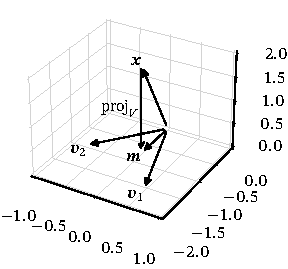
\includegraphics{figures/proj3d.pdf}
  \caption{\(\vect{x}\)の\(V=\spannedby\Set{\vect{v}_1,\vect{v}_2}\)への直交射影\(\vect{m}=\proj_V\vect{x}\)の模式図.}
\end{figure}

\begin{example}
  \(V=\spannedby\Set{\vect{i},\vect{j}}\)(\(\vect{i}=\trps{\rowvect{1 & 0 & 0}}\),\(\vect{j}=\trps{\rowvect{0 & 1 & 0}}\))で\(\numset{R}^3\)の部分空間\(V\)を定める.
  このとき,集合\(\Set{\vect{i},\vect{j}}\)は\(V\)の正規直交基底なので\(\proj_V\vect{r}=\innerp{\vect{r}}{\vect{i}}\vect{i}+\innerp{\vect{r}}{\vect{j}}\vect{j}=\trps{\rowvect{x & y & 0}}\)(\(\vect{r}=\trps{\rowvect{x & y & z}}\))である.
\end{example}

\begin{proposition}{}{}
  \(\numset{K}^n\)の任意の部分空間\(V\)について,写像\(\proj_V\colon\numset{K}^n\to V\)は線型写像である.
\end{proposition}

\begin{proof}
  \(s,t\in\numset{K}\),\(\vect{x},\vect{y}\in\numset{K}^n\)を任意にとり,\(\vect{m}=s\proj_V(\vect{x})+t\proj_V(\vect{y})\),\(\vect{z}=s\vect{x}+t\vect{y}\)とおく.
  このとき,各\(\vect{v}\in V\)に対し\(\innerp{\vect{z}-\vect{m}}{\vect{v}}=s\innerp{\vect{x}-\proj_V\vect{x}}{\vect{v}}+t\innerp{\vect{y}-\proj_V\vect{y}}{\vect{v}}=s0+t0=0\)なので\(\proj_V\vect{z}=\vect{m}\)である.
\end{proof}

\begin{definition}{直交補空間}{numerical_perpendicular_complement}\index{ちょっこうほくうかん@直交補空間}\indexsymbol{\(\pcomp[V]{W}\)}\indexsymbol{\(\pcomp{V}\)}
  \(V\)を\(\numset{K}^n\)の部分空間とする.\(W\)が\(V\)の部分空間なら,集合
  \[
    \Set{\vect{v}\in V\given\text{任意の\(\vect{w}\in W\)に対して\(\innerp{\vect{v}}{\vect{w}}=0\)}}
  \]
  も\(V\)の部分空間になる.この部分空間を(\(V\)における)\(W\)の\termdef{直交補空間}(orthogonal complement)といい,\(\pcomp[V]{W}\),\(\pcomp{W}\)などと書く.
\end{definition}

\begin{example}
  \(W=\spannedby\Set{\vect{e}_1,\vect{e}_2}\)を\(\numset{R}^3\)の2次元部分空間とする.
  このとき,\(\pcomp{W}\)は\(\vect{e}_1\)と\(\vect{e}_2\)に直交し\(\zvec\)でないベクトル\(\vect{e}_3\)が生成する直線\(\spannedby\Set{\vect{e}_3}\)である.
  \(\innerp{\vect{e}_1}{\vect{e}_2}=0\)なら集合\(\Set{\vect{e}_i/\vnorm{\vect{e}_i}\given i=1,2,3}\)は\(\numset{R}^3\)の正規直交基底である.
\end{example}

\begin{figure}[htbp]
  \centering
  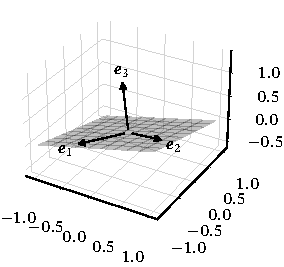
\includegraphics{figures/orthogonal_complement.pdf}
  \caption{\(W\)と\(\vect{e}_1\),\(\vect{e}_2\),\(\vect{e}_3\)の様子.}
\end{figure}

\begin{proposition}{}{}
  \(V\)は\(\numset{K}^n\)の部分空間で,\(W\)は\(V\)の部分空間とする.このとき\(V=W\oplus\pcomp[V]{W}\)である.
\end{proposition}

\begin{proof}
  \(\vect{x}\in W\cap\pcomp{W}\)なら\(\innerp{\vect{x}}{\vect{x}}=0\)より\(\vect{x}=\zvec\)である.
  また,任意の\(\vect{x}\in W\)に対して\(\vect{x}-\proj_W\vect{x}\in\pcomp{W}\),\(\vect{x}=\proj_W(\vect{x})+(\vect{x}-\proj_W\vect{x})\in W+\pcomp{W}\)である.よって\(V=W\oplus\pcomp{W}\)である.
\end{proof}

\subsection{分析と合成}
\label{subsection:analysis_and_synthesis}

\cref{proposition:finite_convex_projection}の証明では,\(\proj_V\vect{x}\)の存在を示すために\(V\)の正規直交基底\(\Set{\vect{e}_1,\dots,\vect{e}_m}\)を1つ選び,\(\proj_V\vect{x}\)を\(\sum_{i=1}^m\innerp{\vect{x}}{\vect{e}_i}\vect{e}_i\)と表した.
一方で,\(\vect{x}\)の性質を調べるのに使いたい\(\numset{C}^n\)の正規直交基底\(\Set{\vect{e}_1,\dots,\vect{e}_n}\)がさきにあって,そこから部分空間\(V_m=\spannedby\Set{\vect{e}_1,\dots,\vect{e}_m}\)(\(m=1,\dots,n\))への直交射影\(\proj_{V_m}\vect{x}\)を作ることも多い.
そのような場合,直交射影は3つの操作に分解できる.

\begin{definition}{エルミート転置}{hermitian_transpose}\index{えるみーとてんち@エルミート転置}\index{ずいはんぎょうれつ@随伴行列|see{エルミート転置}}\index{H@\(\htrps{\mat{A}}\)}
  \(\mat{A}\)を\(m\times n\)複素行列とする.\(n\times m\)行列\(\trps{\conj{\mat{A}}}\)を\(\mat{A}\)の\termdef{エルミート転置}(Hermitian transpose)といい\footnotemark ,\(\htrps{\mat{A}}\)と表す.
\end{definition}

\footnotetext{エルミート転置は\termdef{随伴行列}(adjoint matrix)と呼ばれることも多い.}
\(\mat{U}=\rowvect{\vect{e}_1 & \cdots & \vect{e}_n}\),\(\mat{\Delta}=\smallmatrice{\imat_m & \\ & \zmat_{n-m}}\)とおく(\(\imat_m\)は\(m\)次単位行列,\(\zmat_{n-m}\)は\(n-m\)次零行列).
このとき,任意の\(\vect{x}=\trps{\rowvect{x_1 & \cdots & x_n}}\in\numset{C}^n\)に対して
\[
  \htrps{\mat{U}}\vect{x} = \matrice*{\htrps{\vect{e}_1}\vect{x} \\ \vdots \\ \htrps{\vect{e}_n}\vect{x}}
  = \matrice*{\innerp{\vect{x}}{\vect{e}_1} \\ \vdots \\ \innerp{\vect{x}}{\vect{e}_n}},
  \quad\mat{\Delta}\vect{x} = \matrice*{x_1 \\ \vdots \\ x_m \\ \zvec},
  \quad\mat{U}\vect{x} = \mat{U}\matrice*{x_1 \\ \vdots \\ x_n}
  = \sum_{i=1}^nx_i\vect{e}_i
\]
であるから
\[
  \mat{U}\mat{\Delta}\htrps{\mat{U}}\vect{x} = \mat{U}\mat{\Delta}\matrice*{\innerp{\vect{x}}{\vect{e}_1} \\ \vdots \\ \innerp{\vect{x}}{\vect{e}_n}}
  = \mat{U}\matrice*{\innerp{\vect{x}}{\vect{e}_1} \\ \vdots \\ \innerp{\vect{x}}{\vect{e}_m} \\ \zvec}
  = \sum_{i=1}^m\innerp{\vect{x}}{\vect{e}_i}\vect{e}_i
  = \proj_{V_m}\vect{x}
\]
であり,\(\proj_{V_m}\vect{x}=\mat{U}\mat{\Delta}\htrps{\mat{U}}\vect{x}\)が成立する.よって,\(\proj_{V_m}\)は線型写像\(T(\vect{x})=\htrps{\mat{U}}\vect{x}\),\(D(\vect{x})=\mat{\Delta}\vect{x}\),\(\synth{T}(\vect{x})=\mat{U}\vect{x}\)を用いて\(\proj_{V_m}=\synth{T}DT\)と表せる.

\(T(\vect{x})\)の第\(i\)成分\(\innerp{\vect{x}}{\vect{e}_i}\)は,\(\vect{x}\)に含まれる\(\vect{e}_i\)の「成分」を表すと考えられる.その理由は2つある.
1つめの理由は,\(\vnorm{\proj_{\spannedby\Set{\vect{e}_i}}\vect{x}}=\vnorm{\innerp{\vect{x}}{\vect{e}_i}\vect{e}_i}=\abs{\innerp{\vect{x}}{\vect{e}_i}}\)なので,
\(\abs{\innerp{\vect{x}}{\vect{e}_i}}\)が\(\vect{e}_i\)のスカラー倍で\(\vect{x}\)を最もよく近似するベクトルの長さを表すことである.
もう一つの理由は,\(\basis{B}\)は\(\numset{K}^n\)の正規直交基底であるから
\begin{equation}
  \label{equation:analysis_and_synthesis}
  \vect{x} = \proj_{V_n}\vect{x}
  = \sum_{i=1}^n\innerp{\vect{x}}{\vect{e}_i}\vect{e}_i
\end{equation}
が成立し,\(\innerp{\vect{x}}{\vect{e}_i}\vect{e}_i\)の和で\(\vect{x}\)が表されることである.

以上の理由から,本書では線型写像\(T(\vect{x})=\trps{\rowvect{\innerp{\vect{x}}{\vect{e}_1} & \cdots & \innerp{\vect{x}}{\vect{e}_n}}}\)を分析作用素,\(\synth{T}(\vect{x})=\sum_{i=1}^nx_i\vect{e}_i\)を合成作用素と呼ぶ.

\begin{definition}{分析作用素,合成作用素}{analysis_and_synthesis}\index{ぶんせきさようそ@分析作用素}\index{ごうせいさようそ@合成作用素}
  \(\basis{B}=\Set{\vect{e}_1,\dots,\vect{e}_n}\)を\(\numset{K}^n\)の正規直交基底とする.
  \begin{enumerate}
    \item 線型写像\(T\colon\numset{K}^n\to\numset{K}^n\),\(T(\vect{x})=\trps{\rowvect{\innerp{\vect{x}}{\vect{e}_1} & \cdots & \innerp{\vect{x}}{\vect{e}_n}}}\)を\(\basis{B}\)に関する\termdef{分析作用素}(analysis operator)という.
    \item 線型写像\(\synth{T}\colon\numset{K}^n\to\numset{K}^n\),\(\synth{T}(\trps{\rowvect{x_1 & \cdots & x_n}})=\sum_{i=1}^nx_i\vect{e}_i\)を\(\basis{B}\)に関する\termdef{合成作用素}(synthesis operator)という.
  \end{enumerate}
\end{definition}

\cref{equation:analysis_and_synthesis}より,合成作用素は分析作用素の逆写像である.
また,分析作用素と合成作用素が持つ性質は,表現行列に関する条件へと言い換えられる.

\begin{definition}{正規行列,ユニタリ行列}{regular_and_unitary_matrix}\index{せいきぎょうれつ@正規行列}\index{ぎょうれつ@行列!せいき@正規\texttwoemdash}\index{ゆにたりぎょうれつ@ユニタリ行列}\index{ぎょうれつ@行列!ゆにたり@ユニタリ\texttwoemdash}
  \(\mat{A}\)を\(n\)次複素正方行列とする.
  \begin{enumerate}
    \item \(\htrps{\mat{A}}\mat{A}=\mat{A}\htrps{\mat{A}}\)であるとき,\(\mat{A}\)を\termdef{正規行列}(normal matrix)という.
    \item \(\htrps{\mat{A}}\mat{A}=\mat{A}\htrps{\mat{A}}=\imat\)(つまり\(\htrps{\mat{A}}=\mat{A}^{-1}\))であるとき,\(\mat{A}\)を\termdef{ユニタリ行列}(unitary matrix)という.
  \end{enumerate}
\end{definition}

正規行列については\cref{section:least_square}で詳述するとして,ここでは次の命題を示す.

\begin{proposition}{ユニタリ行列の特徴づけ}{unitary_matrix_characterization}
  \(\mat{U}=\rowvect{\vect{u}_1 & \cdots & \vect{u}_n}\)を\(n\)次複素正方行列とする.このとき,\(\mat{U}\)に関する以下の条件は同値である.
  \begin{enumerate}
    \item \(\mat{U}\)はユニタリ行列である.
    \item 集合\(\Set{\vect{u}_1,\dots,\vect{u}_n}\)は\(\numset{C}^n\)の正規直交基底である.
    \item 任意の\(\vect{x},\vect{y}\in\numset{C}^n\)に対して\(\innerp{\mat{U}\vect{x}}{\mat{U}\vect{y}}=\innerp{\vect{x}}{\vect{y}}\)である.
  \end{enumerate}
\end{proposition}

\begin{proof}
  まず,1と2の同値性を示す.
  \[
    \htrps{\mat{U}}\mat{U} = \matrice*{\htrps{\vect{u}_1} \\ \vdots \\ \htrps{\vect{u}_n}}\matrice{\vect{u}_1 & \cdots & \vect{u}_n}
     = \matrice*{\htrps{\vect{u}_1}\vect{u}_1 & \cdots & \htrps{\vect{u}_1}\vect{u}_n \\ \vdots & \ddots & \vdots \\ \htrps{\vect{u}_n}\vect{u}_1 & \cdots & \htrps{\vect{u}_n}\vect{u}_n}
 \]
  なので,\(\innerp{\vect{u}_i}{\vect{u}_j}=\htrps{\vect{u}_j}{\vect{u}_i}=\kdelta{i}{j}\)がすべての\(i,j\in\Set{1,\dots,n}\)で成り立つことは,\(\htrps{\mat{U}}\mat{U}=\imat\)と同値である.

  次に,3と1の同値性を示す.\(\innerp{\mat{U}\vect{x}}{\mat{U}\vect{y}}=\htrps{(\mat{U}\vect{y})}\mat{U}\vect{x}=\htrps{(\htrps{\mat{U}}\mat{U}\vect{y})}\vect{x}=\innerp{\vect{x}}{\htrps{\mat{U}}\mat{U}\vect{y}}\)なので
  \(\innerp{\vect{x}}{\vect{y}}-\innerp{\mat{U}\vect{x}}{\mat{U}\vect{y}}=\innerp{\vect{x}}{\mat{E}\vect{y}}\)(\(\mat{E}=\imat-\htrps{\mat{U}}\mat{U}\))である.
  任意の\(\vect{x}\in\numset{C}^n\)に対し\(\innerp{\vect{x}}{\mat{E}\vect{y}}=0\)なら,\(\vect{x}=\mat{E}\vect{y}\)とすれば\(\vnorm{\mat{E}\vect{y}}^2=0\),すなわち\(\mat{E}\vect{y}=\zvec\)が得られる.
  \(\mat{E}\vect{y}=\zvec\)がすべての\(\vect{y}\in\numset{C}^n\)で成り立つとき,\(\mat{E}=\zmat\)だから\(\mat{U}\)はユニタリ行列である.
  逆に\(\mat{U}\)がユニタリ行列なら,\(\mat{E}=\zmat\)より\(\innerp{\vect{x}}{\vect{y}}-\innerp{\mat{U}\vect{x}}{\mat{U}\vect{y}}=\innerp{\vect{x}}{\mat{E}\vect{y}}=0\)である.
\end{proof}

\begin{note}
  対象が\kenten{ある}条件を満たし,しかも条件を満たす対象が他にないとき,その条件は対象を\termdef{特徴づける}\index{とくちょうづける@特徴づける}(characterize)という.
  \cref{proposition:unitary_matrix_characterization}から,ユニタリ行列の全体集合は複数の方法で特徴づけられる.しかし,どの方法を採用しても指し示す集合は変わらない.
\end{note}

\begin{corollary}{}{}
  \(T\colon\numset{C}^n\to\numset{C}^n\)を線型写像とする.このとき,\(T\)に関する以下の条件は同値である.
  \begin{enumerate}
    \item \(T\)は\(\numset{C}^n\)のある正規直交基底に関する分析作用素である.
    \item 標準基底に関する\(T\)の表現行列はユニタリ行列である.
  \end{enumerate}
\end{corollary}

\begin{proof}
  \(T\)を正規直交基底\(\basis{B}=\Set{\vect{u}_1,\dots,\vect{u}_n}\)に関する分析作用素とすると,\cref{subsection:analysis_and_synthesis}冒頭の議論から
  \(T(\vect{x})=\htrps{\mat{U}}\vect{x}\)(\(\mat{U}=\rowvect{\vect{u}_1 & \dots & \vect{u}_n}\))である.
  また,\(\basis{B}\)は正規直交基底なので,\cref{proposition:unitary_matrix_characterization}より\(\mat{U}\)は\texttwoemdash よって\(\htrps{\mat{U}}\)も\texttwoemdash ユニタリ行列である.逆の証明は省略する.
\end{proof}

\section{最小2乗法}
\label{section:least_square}

本節では,直交射影の理論を近似へと応用する.

\subsection{最小2乗法}

いまから考えるのは,変数\(\vect{x}=\trps{\rowvect{x_1 & \cdots & x_p}}\)に関する連立1次方程式
\begin{equation}
  \label{equation:linear_equation}
  \matrice*{\midx{a}{1}{1} & \cdots & \midx{a}{1}{p} \\ \vdots & \ddots & \vdots \\ \midx{a}{n}{1} & \cdots & \midx{a}{n}{p}}\matrice*{x_1 \\ \vdots \\ x_p}
  = \matrice*{b_1 \\ \vdots \\ b_n}
\end{equation}
の解き方である.\(\mat{A}=\matfence{\midx{a}{i}{j}}\),\(\vect{b}=\trps{\rowvect{b_1 & \cdots & b_n}}\)とおくと,\cref{equation:linear_equation}は\(\mat{A}\vect{x}=\vect{b}\)と書ける.もし\(n=p\)で\(\mat{A}\)が正則なら,解は\(\vect{x}=\mat{A}^{-1}\vect{b}\)ただ一つである.

\(\mat{A}\)が正則でないとき,\cref{equation:linear_equation}の厳密解があるかどうかは\(\vect{b}\)次第である.
\termdef{最小2乗法}\index{さいしょうにじょうほう@最小2乗法}(least squares method)は,厳密解の代わりに\termdef{残差}\index{ざんさ@残差}(residual)\(\vect{\epsilon}(\vect{x})=\vect{b}-\mat{A}\vect{x}\)のノルム\(\vnorm{\vect{\epsilon(\vect{x})}}\)を最小にする近似解\(\vect{x}\)を見つける手法である.
次の命題から,所望の近似解\(\vect{x}\)は常に存在する.

\begin{proposition}{}{least_square_existence}
  \(\vect{b}\in\numset{K}^n\)かつ,\(\mat{A}\)は\(\numset{K}\)上の\(n\times p\)行列とする.このとき,集合\(\argmin_{\vect{x}\in\numset{K}^p}\vnorm{\vect{\epsilon}(\vect{x})}\)(\(\vect{\epsilon}(\vect{x})=\vect{b}-\mat{A}\vect{x}\))は空でない.
\end{proposition}

\begin{proof}
  線型写像\(T_A\colon\numset{K}^p\to\numset{K}^n\)を\(T_A(\vect{x})=\mat{A}\vect{x}\)で定義する.
  関数\(\vnorm{\vect{\epsilon}(\vect{x})}\)の最小値は\(\min\Set{\vnorm{\vect{b}-\mat{A}\vect{x}}\given\vect{x}\in\numset{K}^p}=\min\Set{\vnorm{\vect{b}-\vect{z}}\given\vect{z}\in\img T_A}\)であり,\(\vnorm{\vect{b}-\vect{z}}\)の値を最小にする\(\vect{z}\in\img T_A\)は\(\proj_{\img T_A}\vect{b}\)ただ一つである.
  よって,\(\argmin_{\vect{x}\in\numset{K}^p}\vnorm{\vect{\epsilon}(\vect{x})}\)は方程式\(\mat{A}\vect{x}=\proj_{\img T_A}\vect{b}\)の解集合である.この方程式は明らかに解をもつから,\(\argmin_{\vect{x}\in\numset{K}^p}\vnorm{\vect{\epsilon}(\vect{x})}\)は空でない.
\end{proof}

上の証明における\(\img T_A\),つまり部分空間\(\Set{\mat{A}\vect{x}\given\vect{x}\in\numset{K}^p}\)を\(\mat{A}\)の\termdef{列空間}\index{れつくうかん@列空間}\index{col@\(\colsp\mat{A}\)}(column space)といい,\(\colsp\mat{A}\)と表す.
\(\mat{A}=\rowvect{\vect{a}_1 & \cdots & \vect{a}_p}\)とおくと
\[
  \mat{A}\vect{x} = \matrice{\vect{a}_1 & \cdots & \vect{a}_p}\matrice*{x_1 \\ \vdots \\ x_p}
  = \sum_{j=1}^px_j\vect{a}_j\quad(\vect{x}=\trps{\rowvect{x_1 & \cdots & x_p}})
\]
だから,\(\colsp\mat{A}\)は\(\mat{A}\)の列ベクトル全体が生成する部分空間でもある.

\begin{example}\label{example:overdetermined}
  \(\mat{A}=\trps{\smallmatrice{4 & 1 & 2 \\ 0 & 3 & 2}}\),\(\vect{b}=\trps{\rowvect{-4 & -6 & 4}}\)とする.
  \(\vect{a}_1=\trps{\rowvect{4 & 1 & 2}}\),\(\vect{a}_2=\trps{\rowvect{0 & 3 & 2}}\)とおくと\(\colsp\mat{A}=\spannedby\Set{\vect{a}_1,\vect{a}_2}\)である.

  \(P=\proj_{\colsp\mat{A}}\)とおく.\(\Set{\vect{a}_1,\vect{a}_2}\)に\nameref{xr-proposition:gram_schmidt}を適用すると
  \(\vect{e}_1=\trps{\rowvect{4 & 1 & 2}}/\sqrt{21}\),\(\vect{e}_2=\trps{\rowvect{-1 & 2 & 1}}/\sqrt{6}\)が得られるので,
  \(P(\vect{b})=\innerp{\vect{b}}{\vect{e}_1}\vect{e}_1+\innerp{\vect{b}}{\vect{e}_2}\vect{e}_2=-2\trps{\rowvect{1 & 1 & 1}}\)である.
  よって,\(\argmin_{\vect{x}\in\numset{R}^2}\vnorm{\vect{b}-\mat{A}\vect{x}}\)は方程式\(\mat{A}\vect{x}=-2\trps{\rowvect{1 & 1 & 1}}\)の解集合\(\Set{\trps{\rowvect{-1/2 & -1/2}}}\)である.
\end{example}

\begin{figure}[htbp]
  \centering
  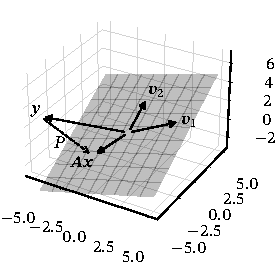
\includegraphics{figures/overdetermined.pdf}
  \caption{\(\vect{a}_1\),\(\vect{a}_2\)と\(P(\vect{b})=\mat{A}\vect{x}\)の様子.}
\end{figure}

\cref{example:overdetermined}からも分かるよう,\(\argmin_{\vect{x}\in\numset{K}^p}\vnorm{\vect{\epsilon}(\vect{x})}\)を求めるには\(\tilde{\vect{b}}=\proj_{\colsp\mat{A}}\vect{b}\)を計算して,方程式\(\mat{A}\vect{x}=\tilde{\vect{b}}\)を解けばよい.
一方で,\(\argmin_{\vect{x}\in\numset{K}^p}\vnorm{\vect{\epsilon}(\vect{x})}\)をより機械的に求める方法もある.

\begin{proposition}{}{normal_equation}
  \(\argmin_{\vect{x}\in\numset{K}^p}\vnorm{\vect{\epsilon}(\vect{x})}=\Set{\vect{x}\in\numset{K}^p\given\htrps{\mat{A}}\mat{A}\vect{x}=\htrps{\mat{A}}\vect{b}}\)である.
\end{proposition}

\begin{proof}
  \(\epsilon(\vect{x})=\vnorm{\vect{\epsilon}(\vect{x})}^2\),\(\increment\epsilon(\vect{x})=\epsilon(\vect{x}+\increment\vect{x})-\epsilon(\vect{x})\)(\(\increment\vect{x}\in\numset{K}^p\))とおくと
  \begin{align*}
    \increment\epsilon(\vect{x}) &= \vnorm{\vect{\epsilon}(\vect{x})-\mat{A}\increment\vect{x}}^2-\vnorm{\vect{\epsilon}(\vect{x})}^2
    = -2\rpart\innerp{\vect{\epsilon}(\vect{x})}{\mat{A}\increment\vect{x}}+\vnorm{\mat{A}\increment\vect{x}}^2 \\
    &= -2\rpart\innerp{\htrps{\mat{A}}(\vect{b}-\mat{A}\vect{x})}{\increment\vect{x}}+\vnorm{\mat{A}\increment\vect{x}}^2
  \end{align*}
  である.よって,\(\numset{K}^p\)の元\(\vect{a}\)が\(\htrps{\mat{A}}\mat{A}\vect{a}=\htrps{\mat{A}}\vect{b}\)を満たすとき,\(\increment\vect{x}\)の値によらず\(\increment\epsilon(\vect{a})=\vnorm{\mat{A}\increment\vect{x}}^2\geq 0\)だから,
  関数\(\epsilon\)は点\(\vect{a}\)で最小値をとる.

  また,\(\increment\vect{x}=h\vect{g}\)(\(h>0\),\(\vect{g}=\htrps{\mat{A}}\vect{b}-\htrps{\mat{A}}\mat{A}\vect{a}\))のとき\(\increment\epsilon(\vect{a})=-2h\vnorm{\vect{g}}^2+h^2\vnorm{\mat{A}\vect{g}}^2\)なので,
  \(\vect{g}=\zvec\)でなければ\(h\)の値が十分小さいとき\(\increment\epsilon(\vect{a})<0\)である.つまり,\(\htrps{\mat{A}}\mat{A}\vect{a}=\htrps{\mat{A}}\vect{b}\)でなければ\(\epsilon(\vect{a})\)は関数\(\epsilon\)の最小値ではない.
\end{proof}

\(\numset{K}^p\)の元\(\vect{x}\)に関する方程式\(\htrps{\mat{A}}\mat{A}\vect{x}=\htrps{\mat{A}}\vect{b}\)を,方程式\(\mat{A}\vect{x}=\vect{b}\)に関する\termdef{正規方程式}\index{せいきほうていしき@正規方程式}(normal equation)という.
\cref{proposition:least_square_existence,proposition:normal_equation}より,もとの方程式が解をもつかどうかによらず,正規方程式の解は存在する.

正規方程式は\cref{proposition:finite_projection}からも導ける.
\(\numset{K}^p\)の元\(\vect{x}\)が\(\mat{A}\vect{x}=\proj_{\colsp\mat{A}}\vect{b}\)を満たすとき,\(\vect{a}_j\in\colsp\mat{A}\)なので\(\innerp{\vect{b}-\mat{A}\vect{x}}{\vect{a}_j}=\htrps{\vect{a}_j}(\vect{b}-\mat{A}\vect{x})=0\)である.
よって\(\htrps{\mat{A}}(\vect{b}-\mat{A}\vect{x})=\zvec\)である.

\subsection{スペクトル分解と特異値分解}
\label{subsection:sd_and_svd}

\(\argmin_{\vect{x}\in\numset{K}^p}\vnorm{\vect{\epsilon}(\vect{x})}\)についてさらに詳しく調べるには,以下の定理が必要である.

\begin{theorem}{スペクトル定理}{spectral_theorem}\index{すぺくとるていり@スペクトル定理}
  \(\mat{A}\)を\(n\)次複素正方行列とする.このとき,\(\mat{A}\)に関する以下の条件は同値である.これを\termdef{スペクトル定理}(spectral theorem)という.
  \begin{enumerate}
    \item \(\mat{A}\)は正規行列である.
    \item \(\mat{A}\)はユニタリ行列で対角化できる.すなわち,\(\mat{A}=\mat{U}\mat{\Lambda}\htrps{\mat{U}}\)を満たす\(n\)次ユニタリ行列\(\mat{U}\),対角行列\(\mat{\Lambda}\)が存在する.
  \end{enumerate}
\end{theorem}

\begin{proof}
  \cref{subsection:proof_of_the_spectral_theorem}を参照せよ(ひとまず認めてもかまわない).
\end{proof}

ユニタリ行列による対角化は\termdef{スペクトル分解}\index{すぺくとるぶんかい@スペクトル分解}(spectral decomposition)と呼ばれる.
\cref{theorem:spectral_theorem}から,正規行列であることとスペクトル分解できることは同値である.

\begin{note}
  正規行列のスペクトル分解を計算するには,固有空間一つ一つの正規直交基底を求め,それらを並べて1つのユニタリ行列を作ればよい.
\end{note}

\begin{corollary}{特異値分解}{singular_value_decomposition}\index{とくいちぶんかい@特異値分解}\index{SVD|see{特異値分解}}
  \(\mat{A}\)を任意の\(n\times p\)複素行列とする.このとき,以下の条件すべてを満たす行列\(\mat{U}\),\(\mat{V}\),\(\mat{\Sigma}\)が存在する.
  式\(\mat{A}=\mat{U}\mat{\Sigma}\htrps{\mat{V}}\)を\(\mat{A}\)の\termdef{特異値分解}(singular value decomposition; SVD)という.
  \begin{enumerate}
    \item \(\mat{A}=\mat{U}\mat{\Sigma}\htrps{\mat{V}}\)である.
    \item \(\mat{U}\)は\(n\)次ユニタリ行列,\(\mat{V}\)は\(p\)次ユニタリ行列である.
    \item \(\mat{\Sigma}\)は\(n\times p\)行列であり\(\mat{\Sigma}=\smallmatrice{\diag(\sigma_1,\dots,\sigma_k) & \\ & \zmat}\)と書ける.
      ただし\(k=\min\Set{n,p}\),\(\sigma_1\geq\dots\geq\sigma_k\geq 0\)である.
  \end{enumerate}
\end{corollary}

\begin{proof}
  \(\mat{A}\neq\zmat\),\(n\geq p\)のときのみ示す.\(\htrps{\mat{A}}\mat{A}\)は\(p\)次正規行列なので,\cref{theorem:spectral_theorem}よりスペクトル分解\(\htrps{\mat{A}}\mat{A}=\mat{V}\mat{\Lambda}\htrps{\mat{V}}\)が存在する.
  \(\mat{V}=\rowvect{\vect{v}_1 & \cdots & \vect{v}_p}\),\(\mat{\Lambda}=\diag(\lambda_1,\dots,\lambda_p)\)とおく.\(\kdelta{i}{j}=\innerp{\vect{v}_i}{\vect{v}_j}=\htrps{\vect{v}_j}\vect{v}_i\),\(\lambda_i\vect{v}_i=(\htrps{\mat{A}}\mat{A})\vect{v}_i\)より
  \begin{equation}
    \label{equation:image_orthogonality}
    \lambda_i\kdelta{i}{j} = \htrps{\vect{v}_j}(\lambda_i\vect{v}_i)
    = \htrps{\vect{v}_j}(\htrps{\mat{A}}\mat{A})\vect{v}_i
    = \htrps{(\mat{A}\vect{v}_j)}\mat{A}\vect{v}_i
    = \innerp{\mat{A}\vect{v}_i}{\mat{A}\vect{v}_j}
  \end{equation}
  だから,各\(\lambda_i=\vnorm{\mat{A}\vect{v}_i}^2\)はすべて非負である.また
  \[
    \htrps{\mat{A}}\mat{A} = \matrice{\vect{v}_1 & \cdots & \vect{v}_p}\matrice*{\lambda_1 & & \\ & \ddots & \\ & & \lambda_p}\matrice*{\htrps{\vect{v}_1} \\ \vdots \\ \htrps{\vect{v}_p}}
    = \sum_{i=1}^p\lambda_i\vect{v}_i\htrps{\vect{v}_i}
  \]
  であり,和の順序を変えても値は変わらない.そこで,\(\lambda_1\geq\dots\geq\lambda_p\)が成り立つように\(\lambda_1,\dots,\lambda_p\)と\(\vect{v}_1,\dots,\vect{v}_p\)を並べ替えておく.

  \(\sigma_i=\sqrt{\lambda_i}=\vnorm{\mat{A}\vect{v}_i}\),\(r=\max\Set{i\given\mat{A}\vect{v}_i\neq\zvec}\)とおく.
  \cref{equation:image_orthogonality}より,\(\vect{u}_i=(1/\sigma_i)\mat{A}\vect{v}_i\)とおくと集合\(\Set{\vect{u}_1,\dots,\vect{u}_r}\)は\(\numset{C}^n\)の正規直交系である.
  \(r<n\)のときは\(\vect{u}_{r+1},\dots,\vect{u}_n\in\numset{C}^n\)を適切に補うことで,集合\(\Set{\vect{u}_1,\dots,\vect{u}_n}\)を\(\numset{C}^n\)の正規直交基底にできる.
  すると,\(\mat{U}=\rowvect{\vect{u}_1 & \cdots & \vect{u}_n}\)はユニタリ行列であり
  \[
    \htrps{\mat{U}}(\mat{A}\mat{V}) = \htrps{\mat{U}}\matrice{\sigma_1\vect{u}_1 & \cdots & \sigma_r\vect{u}_r & \zmat}
    = \matrice*{\diag(\sigma_1,\dots,\sigma_r) & \\ & \zmat}
  \]
  が成り立つ.\(\sigma_{r+1}=\dots=\sigma_k=0\)なので,右辺の行列は\(\smallmatrice{\diag(\sigma_1,\dots,\sigma_k) & \\ & \zmat}\)と表せる.
  この行列を\(\mat{\Sigma}\)とおくと\(\mat{A}=\mat{U}\mat{\Sigma}\htrps{\mat{V}}\)である.
\end{proof}

\(\mat{A}\)の特異値分解が\(\mat{A}=\mat{U}\smallmatrice{\diag(\sigma_1,\dots,\sigma_k) & \\ & \zmat}\htrps{\mat{V}}\)であるとき,
各\(\sigma_i\)を\(\mat{A}\)の第\(i\)\termdef{特異値}\index{とくいち@特異値}(singular value)という.

特異値分解に基づいて\(\argmin_{\vect{x}\in\numset{C}^p}\vnorm{\vect{\epsilon}(\vect{x})}\)を求めよう.
\(\mat{A}\neq\zmat\)を仮定し,\(\mat{A}\)の特異値分解を\(\mat{A}=\mat{U}\mat{\Sigma}\htrps{\mat{V}}\)とおく.
\cref{proposition:unitary_matrix_characterization}から,ユニタリ行列を掛けてもノルムは変わらないので
\(\vnorm{\vect{\epsilon}(\vect{x})}^2=\vnorm{\vect{b}-\mat{U}\mat{\Sigma}\htrps{\mat{V}}\vect{x}}^2=\vnorm{\htrps{\mat{U}}\vect{b}-\mat{\Sigma}\htrps{\mat{V}}\vect{x}}^2\)である.
\(\vect{y}=\trps{\rowvect{y_1 & \cdots & y_p}}=\htrps{\mat{V}}\vect{x}\),\(\mat{U}=\rowvect{\vect{u}_1 & \cdots & \vect{u}_n}\),\(\mat{\Sigma}=\smallmatrice{\diag(\sigma_1,\dots,\sigma_r) & \\ & \zmat}\)(\(\sigma_r>0\))とおくと
\[
  \vnorm{\vect{\epsilon}(\vect{x})}^2 = \vnorm{\htrps{\mat{U}}\vect{b}-\mat{\Sigma}\vect{y}}^2
  = \sum_{i=1}^r\abs{\htrps{\vect{u}_i}\vect{b}-\sigma_iy_i}^2+\sum_{i=r+1}^p\abs{\htrps{\vect{u}_i}\vect{b}}^2
\]
となる.右辺の値が最も小さくなるのは\(y_i=\htrps{\vect{u}_i}\vect{b}/\sigma_i\)(\(1\leq i\leq r\))のときであり,\(y_{r+1},\dots,y_p\)の値はなんであっても構わない.
\(\vect{x}=\mat{V}\vect{y}\)だから,\(\vnorm{\vect{\epsilon}(\vect{x})}\)が最小値をとるのは\(\vect{x}\)が
\[
  \vect{x} = \mat{V}\trps{\matrice{\htrps{\vect{u}_1}\vect{b}/\sigma_1 & \cdots & \htrps{\vect{u}_r}\vect{b}/\sigma_r & z_{r+1} & \cdots & z_p}}\quad(z_i\in\numset{C})
\]
と表せるときである.\(\vect{z}=\trps{\rowvect{z_1 & \cdots & z_p}}\),\(\pinv{\mat{\Sigma}}=\smallmatrice{\diag(1/\sigma_1,\dots,1/\sigma_r) & \\ & \zmat}\),\(\pinv{\mat{A}}=\mat{V}\pinv{\mat{\Sigma}}\htrps{\mat{U}}\)とおいて整理すると,
\(\pinv{\mat{\Sigma}}\mat{\Sigma}=\smallmatrice{\imat_r & \\ & \zmat_{p-r}}\)なので
\begin{align*}
  \vect{x} &= \mat{V}\matrice*{(1/\sigma_1)\htrps{\vect{u}_1}\vect{b} \\ \vdots \\ (1/\sigma_r)\htrps{\vect{u}_r}\vect{b} \\ \zvec_{p-r}}+\mat{V}\matrice*{\zvec_r \\ z_{r+1} \\ \vdots \\ z_p}
  = \mat{V}\pinv{\mat{\Sigma}}\htrps{\mat{U}}\vect{b}+\mat{V}(\imat-\pinv{\mat{\Sigma}}\mat{\Sigma})\vect{z} \\
  &= \pinv{\mat{A}}\vect{b}+(\imat-\mat{V}\pinv{\mat{\Sigma}}\mat{\Sigma}\htrps{\mat{V}})\mat{V}\vect{z}
  = \pinv{\mat{A}}\vect{b}+(\imat-\pinv{\mat{A}}\mat{A})\vect{w}
\end{align*}
である(ただし\(\vect{w}=\mat{V}\vect{z}\)).\(\pinv{\mat{A}}\)を\(\mat{A}\)の擬似逆行列という.

\begin{definition}{擬似逆行列}{}\index{むーあぺんろーずぎゃくぎょうれつ@ムーア・ペンローズ逆行列}\index{ぎじぎゃくぎょうれつ@擬似逆行列}\indexsymbol{\(\pinv{\mat{A}}\)}
  \(\mat{A}\)を\(n\times p\)複素行列とし,\(\mat{A}\)の特異値分解を\(\mat{A}=\mat{U}\mat{\Sigma}\htrps{\mat{V}}\)とおく.
  \(p\times n\)行列\(\pinv{\mat{\Sigma}}\)を次のように定義する.\(\mat{A}=\zmat\)のときは\(\pinv{\mat{\Sigma}}=\zmat\)とする.
  \(\mat{A}\neq\zmat\)のときは,\(\mat{\Sigma}=\smallmatrice{\mat{\Delta} & \\ & \zmat}\)を満たす正則な対角行列\(\mat{\Delta}\)を用いて\(\pinv{\mat{\Sigma}}=\smallmatrice{\mat{\Delta}^{-1} & \\ & \zmat}\)とする.
  \(p\times n\)行列\(\pinv{\mat{A}}=\mat{V}\pinv{\mat{\Sigma}}\htrps{\mat{U}}\)を\(\mat{A}\)の\termdef{ムーア・ペンローズ逆行列}(Moore–Penrose inverse),あるいは\termdef{擬似逆行列}(pseudoinverse)という.
\end{definition}

\begin{note}
  普通,特異値分解はもとの行列に対して一意ではない.しかし,擬似逆行列はもとの行列に対して一意に定まる.このことは\cref{subsection:pseudoinverse}で示す.
\end{note}

さきほどの議論から分かることは,擬似逆行列によって次のようにまとめられる.

\begin{proposition}{}{pseudoinverse_least_square}
  任意の\(n\times p\)複素行列\(\mat{A}\)に対して,次の式が成立する.
  \[
    \argmin_{\vect{x}\in\numset{C}^p}\vnorm{\vect{b}-\mat{A}\vect{x}} = \Set{\pinv{\mat{A}}\vect{b}+(\imat-\pinv{\mat{A}}\mat{A})\vect{w}\given\vect{w}\in\numset{C}^p}\quad(\vect{b}\in\numset{C}^n)
  \]
\end{proposition}

\subsection{擬似逆行列と解の構造}
\label{subsection:pseudoinverse}

これまでと同様,\(\mat{A}\)は任意の\(n\times p\)複素行列,\(\vect{b}\)は\(\numset{C}^n\)の任意の元とする.
ここでは擬似逆行列の性質と\(\argmin_{\vect{x}\in\numset{C}^p}\vnorm{\vect{b}-\mat{A}\vect{x}}\)の構造について説明する.

\begin{proposition}{擬似逆行列の特徴づけ}{pseudoinverse_characterization}
  以下の条件すべてを満たす\(p\times n\)行列\(\mat{X}\)は,\(\mat{A}\)に対し一意である.
  また,\(\mat{A}\)の擬似逆行列は条件を満たす.つまり,以下の条件は\(\mat{X}=\pinv{\mat{A}}\)と同値である.
  \begin{enumerate}
    \item \(\mat{A}\mat{X}\mat{A}=\mat{A}\)
    \item \(\mat{X}\mat{A}\mat{X}=\mat{X}\)
    \item \(\htrps{(\mat{A}\mat{X})}=\mat{A}\mat{X}\)
    \item \(\htrps{(\mat{X}\mat{A})}=\mat{X}\mat{A}\)
  \end{enumerate}
\end{proposition}

\begin{proof}
  一意性のみ示す.\(p\times n\)行列\(\mat{X}\),\(\mat{Y}\)が条件をすべて満たすとき,\(i\)番目の条件から分かる等号を\(\overset{i}{=\joinrel=}\)と書くと
  \begin{align*}
    \mat{Y} &\overset{2,3}{=\joinrel=} \mat{Y}\htrps{(\mat{A}\mat{Y})}
    = \mat{Y}\htrps{\mat{Y}}\htrps{\mat{A}}
    \overset{1}{=\joinrel=} \mat{Y}\htrps{\mat{Y}}\htrps{(\mat{A}\mat{X}\mat{A})}
    = \mat{Y}\htrps{(\mat{A}\mat{Y})}\htrps{(\mat{A}\mat{X})} \\
    &\overset{2,3}{=\joinrel=} \mat{Y}\mat{A}\mat{X}
    \overset{2,4}{=\joinrel=} \htrps{(\mat{Y}\mat{A})}\mat{X}\mat{A}\mat{X}
    \overset{4}{=\joinrel=} \htrps{\mat{A}}\htrps{\mat{Y}}\htrps{(\mat{X}\mat{A})}\mat{X}
    = \htrps{(\mat{A}\mat{Y}\mat{A})}\htrps{\mat{X}}\mat{X} \\
    &\overset{1}{=\joinrel=} \htrps{\mat{A}}\htrps{\mat{X}}\mat{X}
    = \htrps{(\mat{X}\mat{A})}\mat{X}
    \overset{2,4}{=\joinrel=} \mat{X}
  \end{align*}
  なので\(\mat{Y}=\mat{X}\)である.
\end{proof}

\begin{proposition}{}{pseudoinverse_minimum_norm}
  集合\(S=\argmin_{\vect{x}\in\numset{C}^p}\vnorm{\vect{b}-\mat{A}\vect{x}}\)の元でノルムが最も小さいものは,\(\pinv{\mat{A}}\vect{b}\)ただ一つである.
  すなわち\(\argmin_{\vect{x}\in S}\vnorm{\vect{x}}=\Set{\pinv{\mat{A}}\vect{b}}\)である.
\end{proposition}

\begin{proof}
  \cref{proposition:pseudoinverse_least_square}より\(S\)の任意の元は\(\vect{x}=\pinv{\mat{A}}\vect{b}+\vect{n}\)(\(\vect{n}=(\imat-\pinv{\mat{A}}\mat{A})\vect{w}\))と書けて,
  \cref{proposition:pseudoinverse_characterization}から\(\innerp{\pinv{\mat{A}}\vect{b}}{\vect{n}}=\innerp{(\imat-\pinv{\mat{A}}\mat{A})\pinv{\mat{A}}\vect{b}}{\vect{w}}=0\)である.
  よって\(\vnorm{\vect{x}}^2=\vnorm{\pinv{\mat{A}}\vect{b}}^2+\vnorm{\vect{n}}^2\)なので,\(\argmin_{\vect{x}\in S}\vnorm{\vect{x}}=\Set{\pinv{\mat{A}}\vect{b}}\)である.
\end{proof}

実は,\cref{proposition:pseudoinverse_minimum_norm}において\(\argmin_{\vect{x}\in S}\vnorm{\vect{x}}\)の元が唯一であることは擬似逆行列を使わず証明できる.
\cref{section:least_square}の初めに述べた通り,\(\argmin_{\vect{x}\in\numset{K}^p}\vnorm{\vect{b}-\mat{A}\vect{x}}\)は方程式\(\mat{A}\vect{x}=\tilde{\vect{b}}\)(\(\tilde{\vect{b}}=\proj_{\colsp\mat{A}}\vect{b}\))の解集合である.
この方程式の解を1つ選び\(\vect{a}\)とおくと,他の解\(\vect{x}\)は\(\mat{A}(\vect{x}-\vect{a})=\tilde{\vect{b}}-\tilde{\vect{b}}=\zvec\),
つまり\(\vect{x}-\vect{a}\in\nulsp\mat{A}\)(\(\nulsp\mat{A}=\Set{\vect{n}\in\numset{C}^p\given\mat{A}\vect{n}=\zvec}\))\index{nul@\(\nulsp\mat{A}\)}を満たす.

逆に,\(\numset{K}^p\)の元\(\vect{x}\)が\(\vect{x}-\vect{a}\in\nulsp\mat{A}\)を満たせば\(\mat{A}\vect{x}=\tilde{\vect{b}}\)も成立する.
つまり\(\argmin_{\vect{x}\in\numset{K}^p}\vnorm{\vect{b}-\mat{A}\vect{x}}\)は,部分空間\(\nulsp\mat{A}\)を\(\vect{a}\)によって平行移動した集合\(\Set{\vect{a}+\vect{n}\given\vect{n}\in\nulsp\mat{A}}\)である.
このような集合をアフィン部分空間という.

\begin{definition}{アフィン部分空間}{affine_subspace}\index{あふぃんぶぶんくうかん@アフィン部分空間}\index{ぶぶんくうかん@部分空間!あふぃん@アフィン\texttwoemdash}
  \(S\)をベクトル空間\(V\)の部分集合とする.ある\(\vect{a}\in S\)に対して集合\(W=\Set{\vect{x}-\vect{a}\given\vect{x}\in S}\)が\(V\)の部分ベクトル空間であるとき,
  \(S\)は\(V\)の\termdef{アフィン部分空間}(affine subspace)であるという.このとき\(S\)を\(S=\vect{a}+W\)と表す.
\end{definition}

\begin{figure}[htbp]
  \centering
  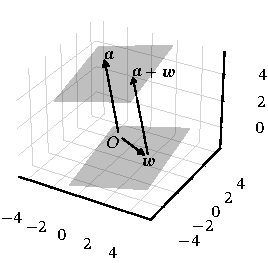
\includegraphics{figures/affine.pdf}
  \caption{アフィン部分空間\(\vect{a}+W\)の模式図.}
\end{figure}

任意の\(\vect{x}\in\numset{K}^p\)とアフィン部分空間\(S\subseteq\numset{K}^p\)に対し,\(\argmin_{\vect{y}\in S}\vnorm{\vect{x}-\vect{y}}\)は\(S\)が部分ベクトル空間のときと同様,ただ一つの元を持つ.
実際,\(S=\vect{a}+W\)(\(\vect{a}\in S\))とおくと\(\argmin_{\vect{y}\in S}\vnorm{\vect{x}-\vect{y}}=\argmin_{\vect{y}-\vect{a}\in W}\vnorm{(\vect{x}-\vect{a})-(\vect{y}-\vect{a})}=\Set{\vect{a}+\proj_W(\vect{x}-\vect{a})}\)である.

よって,集合\(\argmin_{\vect{x}\in S}\vnorm{\vect{x}}\)(\(S=\vect{a}+\nulsp\mat{A}\))も元をただ一つ持つ.そして\cref{proposition:pseudoinverse_minimum_norm}から,その元とは\(\pinv{\mat{A}}\vect{b}\)のことである.

\subsection{\texorpdfstring{\(\numset{K}=\numset{R}\)}{K=R}の場合}

\cref{subsection:sd_and_svd}から\cref{subsection:pseudoinverse}の結果は,スペクトル分解と特異値分解を次の形で適当に読み替えれば\(\numset{K}=\numset{R}\)のときも適用できる.
証明は\(\numset{K}=\numset{C}\)のときとほとんど変わらない.

\begin{theorem}{スペクトル定理}{spectral_theorem_in_real}\index{すぺくとるていり@スペクトル定理!じつぎょうれつ@実行列}\index{ちょっこうぎょうれつ@直交行列}\index{ぎょうれつ@行列!ちょっこう@直交\texttwoemdash}
  \(\mat{A}\)を\(n\)次実正方行列とする.このとき,\(\mat{A}\)に関する以下の条件は同値である.
  \begin{enumerate}
    \item \(\mat{A}\)は正規行列である.
    \item \(\mat{A}\)は直交行列\footnotemark で対角化できる.すなわち,\(\mat{A}=\mat{U}\mat{\Lambda}\trps{\mat{U}}\)を満たす\(n\)次直交行列\(\mat{U}\),対角行列\(\mat{\Lambda}\)が存在する.
  \end{enumerate}
\end{theorem}

\begin{corollary}{特異値分解}{singular_value_decomposition_in_real}\index{とくいちぶんかい@特異値分解!じつぎょうれつ@実行列}
  \(\mat{A}\)を任意の\(n\times p\)実行列とする.このとき,以下の条件すべてを満たす行列\(\mat{U}\),\(\mat{V}\),\(\mat{\Sigma}\)が存在する.
  \begin{enumerate}
    \item \(\mat{A}=\mat{U}\mat{\Sigma}\trps{\mat{V}}\)である.
    \item \(\mat{U}\)は\(n\)次直交行列,\(\mat{V}\)は\(p\)次直交行列である.
    \item \(\mat{\Sigma}\)は\(n\times p\)行列であり\(\mat{\Sigma}=\smallmatrice{\diag(\sigma_1,\dots,\sigma_k) & \\ & \zmat}\)と書ける.
      ただし\(k=\min\Set{n,p}\),\(\sigma_1\geq\dots\geq\sigma_k\geq 0\)である.
  \end{enumerate}
\end{corollary}

\footnotetext{\(\mat{Q}\trps{\mat{Q}}=\trps{\mat{Q}}\mat{Q}=\imat\)を満たす実正方行列\(\mat{Q}\)を\termdef{直交行列}(orthogonal matrix)という.}

\subsection{曲線あてはめ}
\label{subsection:curve_fitting}

ここまで説明した最小2乗法の理論は,データを曲線にあてはめるとき威力を発揮する.

変数\(x\)と変数\(y\)の間には,多項式で表される関係\(y=c_0+c_1x+\dots+c_px^p\)があると仮定する.
次数\(p\)は既知であり,各\(x^k\)の係数\(c_k\)を\(y\)の観測値から推定したい.

たとえば,おもりを自由落下させると落下時間\(t\)と移動距離\(y\)の間には\(y=(g/2)t^2\)という関係がある(\(g\)は重力加速度と呼ばれる定数である).
そこで,\(t\)の値を変えながら\(y\)の値をくり返し測定し,得られたデータを式\(y=at^2\)にあてはめれば,\(g=2a\)の値を間接的に測定できる.

以下では,\(x=x_i\)に対応する観測値\(y_i\)の系列\(y_1,\dots,y_n\)を\(y\)の標本と呼ぶ.
次の定理から,\(c_0,\dots,c_p\)を決定するには最低限\(p+1\)個の標本があればよい.

\begin{theorem}{}{}\index{ほかんたこうしき@補間多項式}
  点列\((x_1,y_1),\dots,(x_{p+1},y_{p+1})\in\numset{K}^2\)は,相異なる任意の\(i,j\in\Set{1,\dots,p+1}\)に対して\(x_i\neq x_j\)を満たすとする.
  このとき,すべての\(i\)で\(f(x_i)=y_i\)を満たす,次数が\(p\)以下の\(\numset{K}\)係数多項式\(f(x)\)がただ一つ存在する\footnotemark .
\end{theorem}

\begin{proof}
  まず\(f(x)\)が存在することを示す.
  \[
    l_k(x) = (x-x_1)(x-x_2)\dotsm(x-x_{k-1})(x-x_{k+1})\dotsm(x-x_{p+1})
  \]
  とおくと\(l_k(x_k)\neq 0\),\(l_k(x_i)=0\)(\(i\neq k\))より\(l_k(x_i)/l_k(x_k)=\kdelta{k}{i}\)である.
  よって,\(f(x)=\sum_{k=1}^{p+1}y_kl_k(x)/l_k(x_k)\)は条件を満たす\(\numset{K}\)係数多項式である.

  次に\(f(x)\)が一意であることを示す.多項式\(f_1(x)\)と\(f_2(x)\)はどちらも条件を満たすとする.
  このとき,多項式\(\delta(x)=f_1(x)-f_2(x)\)は\(\delta(x_i)=y_i-y_i=0\)を満たすので,\(\delta(x)=q(x)(x-x_1)\dotsm(x-x_{p+1})\)と因数分解できる.
  \(\delta(x)\)の次数は最大でも\(p\)だから\(q(x)=0\),すなわち\(f_1(x)=f_2(x)\)である.
\end{proof}

\begin{wrapfigure}[8]{o}{0pt}
  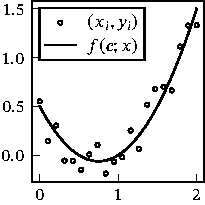
\includegraphics{figures/regression.pdf}
\end{wrapfigure}

\footnotetext{この多項式を\termdef{補間多項式}(interpolating polynomial)という.}
実験で得られるデータは誤差を含むものだから,普通は標本数\(n\)を\(p+1\)より十分に大きくとり,
多項式関数\(f(\vect{c};x)=\sum_{k=0}^pc_kx^k\)のあてはまりが平均的によくなる係数\(\vect{c}=\trps{\rowvect{c_0 & \cdots & c_p}}\)を求める.
図は\(p=2\)における標本と\(f(\vect{c};x)=c_0+c_1x+c_2x^2\)の例である.

あてはまりのよさを評価する指標はいろいろ考えられるが,ここでは関数
\begin{equation}
  \label{equation:mean_square}
  \epsilon(\vect{c}) = \sum_{i=1}^n\abs{y_i-f(\vect{c};x_i)}^2
\end{equation}
を採用する.各\(f(\vect{c};x_i)\)の値が\(y_i\)の値に近いほど\(\epsilon(\vect{c})\)の値は小さくなるので,\(\epsilon(\vect{c})\)の値が小さいほど\(f(\vect{c};x)\)は標本によくあてはまっているといえる.

\begin{note}
  \cref{equation:mean_square}の指標を\termdef{残差平方和}\index{ざんさへいほうわ@残差平方和}\index{RSS|see{残差平方和}}(residual sum of squares; RSS)という.
  RSSであてはまりのよさを測るのが妥当かどうかは,データの性質や分析する目的にもよる.
  しかし,ほかの指標に関して\(\argmin\)を計算するのは\texttwoemdash 空集合でないことを保証するだけでも\texttwoemdash 難しいことが多い.まずはRSSが使えないか考えるべきだろう.
\end{note}

\(\vect{\phi}_i=\trps{\rowvect{x_i^0 & \cdots & x_i^p}}\),\(\mat{\Phi}=\trps{\rowvect{\vect{\phi}_1 & \cdots & \vect{\phi}_n}}\)とおくと,\(f(\vect{c};x_i)=\trps{\vect{\phi}_i}\vect{c}\)だから
\[
  \epsilon(\vect{c}) = \vnorm*{\matrice*{y_1 \\ \vdots \\ y_n}-\matrice*{\trps{\vect{\phi}_1} \\ \vdots \\ \trps{\vect{\phi}_n}}\vect{c}}^2
  = \vnorm{\vect{y}-\mat{\Phi}\vect{c}}^2\quad(\vect{y}=\trps{\matrice{y_1 & \cdots & y_n}})
\]
である.よって,\(f(\vect{c};x)\)が標本に最もよくあてはまる\(\vect{c}\)を求めるには,さきほど示した方法で\(\argmin_{\vect{c}\in\numset{K}^{p+1}}\vnorm{\vect{y}-\mat{\Phi}\vect{c}}\)を計算すればよい.

\begin{example}
  \label{example:linear_regression}
  \(p=1\),\(n=3\),\((x_1,y_1)=(1,0)\),\((x_2,y_2)=(2,3)\),\((x_3,y_3)=(3,1)\)とする.
  \(\mat{\Phi}=\trps{\smallmatrice{1 & 1 & 1 \\ 1 & 2 & 3}}\)とおくと,方程式\(\mat{\Phi}\vect{c}=\vect{y}\)(\(\vect{y}=\trps{\rowvect{0 & 3 & 1}}\))に関する正規方程式は
  \(\trps{\mat{\Phi}}\mat{\Phi}\vect{c}=\trps{\mat{\Phi}}\vect{y}\),\(\smallmatrice{3 & 6 \\ 6 & 14}\vect{c}=\smallmatrice{4 \\ 9}\)である.
  この解は\(\vect{c}=\smallmatrice{1/3 \\ 1/2}\)なので,\(f(\vect{c};x)=1/3+(1/2)x\)のとき\(f(\vect{c};x)\)は標本に最もよくあてはまる.
\end{example}

\begin{figure}[htbp]
  \centering
  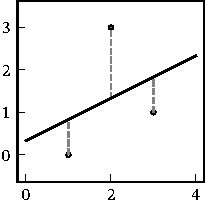
\includegraphics{figures/linear_regression.pdf}
  \caption{\cref{example:linear_regression}の標本と\(f(\vect{c};x)\)の様子.\(\epsilon(\vect{c})\)は破線の長さの平方和である.}
\end{figure}

同じ考え方は,\(y\)が\(x\)の多項式関数でなくても使える.変数\(y\)は,変数\(x\)を既知の関数\(\vect{\phi}(x)=\trps{\rowvect{\phi_1(x) & \cdots & \phi_p(x)}}\)で写像した線型結合によって
\begin{equation}
  \label{equation:linear_combination_of_functions}
  y = c_1\phi_1(x)+\dots+c_p\phi_p(x)
  = \trps{\vect{c}}\vect{\phi}(x)
\end{equation}
と書けるとする.関数\(\epsilon(\vect{c})=\sum_{i=1}^n\abs{y_i-f(\vect{c};x_i)}^2\)(\(f(\vect{c};x)=\sum_{k=1}^pc_k\phi_k(x)\))が最小値をとる\(\vect{c}\in\numset{K}^p\)全体は,集合\(\argmin_{\vect{c}\in\numset{K}^p}\vnorm{\vect{y}-\mat{\Phi}\vect{c}}\)である.
ただし,\(\mat{\Phi}\)は\(n\times p\)行列\(\mat{\Phi}=\trps{\rowvect{\vect{\phi}(x_1) & \cdots & \vect{\phi}(x_n)}}\)である.

なお,\(\phi_1,\dots,\phi_p\)が線型従属だと\cref{equation:linear_combination_of_functions}を満たす\(c_1,\dots,c_p\)の値は一意に定まらない.
そのため,しばしば\(\phi_1,\dots,\phi_p\)は線型独立になるよう設計される.

\section{離散フーリエ変換}
\label{section:dft}

\cref{section:dft}から,本書の主題である信号解析に入る.その手始めに,いまから扱う信号とは何か明確にしておく.

ごくごく一般的に言うと,信号とは入力に対して出力が観測されるもの全般を指し,入力全体\(I\)から出力全体\(O\)への写像でモデル化できる.
たとえば,対象が音声信号なら\(I\)は時刻全体,\(O\)は瞬時値全体である.また,対象がモノクロ画像なら\(I\)は画素の位置全体,\(O\)は白黒の階調全体である.

始域が\(X\),終域が\(Y\)である写像の全体集合は通常\(\mapset{X}{Y}\)\indexsymbol{\(\mapset{X}{Y}\)}と書かれる.
\(I\)と\(O\)を決めたとき,考えられる信号の最も広い枠組みは\(\mapset{I}{O}\)であろう.
しかし,\(\mapset{I}{O}\)の元すべてに共通する特徴は普通そう多くない.
そこで我々は,\(\mapset{I}{O}\)の中でも性質がよい元に限って,それらが持つ特徴を調べる.

\cref{chapter:numerical_vector_space}で扱うのは,\(I\)が整数か\kenten{その}組からなる信号である.
こうした信号を\termdef{離散信号}\index{りさんしんごう@離散信号}\index{しんごう@信号!りさん@離散\texttwoemdash}(discrete signal)という.
反対に,\(I\)が区間\(\ccival{-\krez}{\krez}\)や\(\numset{R}\)のように連続的である信号は\termdef{連続信号}\index{れんぞくしんごう@連続信号}\index{しんごう@信号!れんぞく@連続\texttwoemdash}(continuous signal)という.

時間\(N\)が有限な離散信号の全体\(\mapset{\Set{0,\dots,N-1}}{\numset{K}}\)は,数ベクトル空間\(\numset{K}^N\)と同一視できる.
これは対応\(x=\seq{x_n}_{n=0}^{N-1}\longleftrightarrow\vect{x}=\trps{\rowvect{x_0 & \cdots & x_{N-1}}}\)を考えれば明らかであろう.
また,数列全体\(\mapset{\numset{Z}}{\numset{K}}\)\texttwoemdash これを\termdef{数列空間}\index{すうれつくうかん@数列空間}(sequence space)という\texttwoemdash も,次の演算でベクトル空間になる.
\[
  \seq{x_n}+\seq{y_n} = \seq{x_n+y_n},
  \quad\lambda\seq{x_n} = \seq{\lambda x_n}\quad\text{(\(\seq{x_n},\seq{y_n}\in\mapset{\numset{Z}}{\numset{K}}\),\(\lambda\in\numset{K})\)}
\]

以上を踏まえて,まずは\(\numset{C}^N\)に属する信号の理論を構成しよう.

\subsection{離散フーリエ変換}

\begin{definition}{離散フーリエ変換}{discrete_fourier_transform}\index{りさんふーりえへんかん@離散フーリエ変換!かずべくとる@数ベクトル}\index{DFT|see{離散フーリエ変換}}\index{FZN@\(\dft{N}\)}
  \(\vect{x}=\trps{\rowvect{x_0 & \cdots & x_{N-1}}}\in\numset{C}^N\)とする.
  \[
    \dft{N}\vect{x} = \trps{\matrice{\hat{x}_0 & \cdots & \hat{x}_{N-1}}},
    \quad\hat{x}_k = \frac{1}{\sqrt{N}}\sum_{n=0}^{N-1}x_n\napr^{-2\krez\iuni kn/N}
  \]
  で定義される線型写像\(\dft{N}\colon\numset{C}^N\to\numset{C}^N\)を\termdef{離散フーリエ変換}(Discrete Fourier transform; DFT)という.
\end{definition}

以下では\(\napr^{2\krez\iuni/N}=\cos(2\krez/N)+\iuni\sin(2\krez/N)\)を単に\(\zeta\)と書く.

\begin{proposition}{}{dft_onb}
  \(\vect{w}_k=N^{-1/2}\trps{\rowvect{\zeta^{k\cdot 0} & \cdots & \zeta^{k(N-1)}}}\)とする.
  このとき,集合\(\Set{\vect{w}_0,\dots,\vect{w}_{N-1}}\)は\(\numset{C}^N\)の正規直交基底である.
\end{proposition}

\begin{proof}
  \(\conj{\zeta}=\zeta^{-1}\)だから,\(\innerp{\vect{w}_i}{\vect{w}_j}=\trps{\vect{w}_i}\conj{\vect{w}}_j\)は
  \[
    \sum_{n=0}^{N-1}\frac{\zeta^{in}}{\sqrt{N}}\frac{\conj{\zeta}^{jn}}{\sqrt{N}} = \frac{1}{N}\sum_{n=0}^{N-1}\zeta^{(i-j)n}
    = \begin{cases}(\zeta^{(i-j)N}-1)/(N(\zeta^{i-j}-1)) & (i\neq j), \\ 1 & (i=j)\end{cases}
  \]
  と変形できる.\(\zeta^N=1\)なので\(\innerp{\vect{w}_i}{\vect{w}_j}=\kdelta{i}{j}\)である.
\end{proof}

\cref{proposition:dft_onb}から,\(\dft{N}\)は正規直交基底\(\basis{W}=\Set{\vect{w}_0,\dots,\vect{w}_{N-1}}\)に関する分析作用素である.
分析作用素の逆写像は合成作用素なので,\(\dft{N}\)の逆変換は
\begin{equation}
  \label{equation:idft}
  \vect{x} = \sum_{k=0}^{N-1}\hat{x}_k\vect{w}_k,
  \quad x_n = \frac{1}{\sqrt{N}}\sum_{k=0}^{N-1}\hat{x}_k\napr^{2\krez\iuni kn/N}
\end{equation}
と書ける.

他の諸性質を導く前に,離散フーリエ変換の工学的重要性を見ておこう.

\begin{figure}[htbp]
  \begin{minipage}{\linewidth/2}
    \centering
    \begin{minipage}[t][45mm][c]{\linewidth}
      \centering
      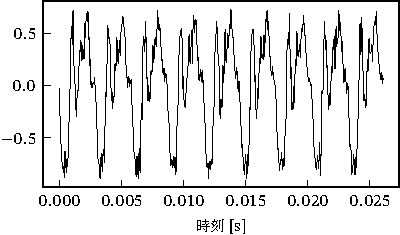
\includegraphics{figures/time_domain.pdf}
    \end{minipage}
    \caption{「あ」の波形.}
    \label{figure:time_domain}
  \end{minipage}%
  \begin{minipage}{\linewidth/2}
    \centering
    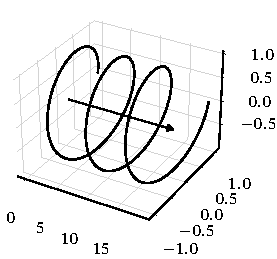
\includegraphics{figures/helix.pdf}
    \caption{複素指数関数のグラフ.}
    \label{figure:complex_sinusoid}
  \end{minipage}
\end{figure}

\cref{figure:time_domain}は「あ」という音声の波形である\footnote{カノン\cite{canon}による波音リツ単独音バージョン1.5.1を使用した.}.
冒頭で述べたように,\cref{figure:time_domain}のデータは数ベクトル\(\vect{x}\in\numset{C}^N\)と見なせる.
そして,分析作用素に関する考察によれば,\(\hat{x}_k=\innerp{\vect{x}}{\vect{w}_k}\)は\(\vect{x}\)に含まれる\(\vect{w}_k\)の成分に相当する.
つまり,\(\hat{x}_k\)の絶対値\(\abs{\hat{x}_k}\)は音声\(\vect{x}\)に含まれる\(\vect{w}_k\)の量を表すと考えられる.では,偏角\(\arg\hat{x}_k\)はどういう意味を持つのだろう\?極形式\(\hat{x}_k=\abs{\hat{x}_k}\napr^{\iuni\arg\hat{x}_k}\)を\cref{equation:idft}に代入すると
\[
  x_n = \frac{1}{\sqrt{N}}\sum_{k=0}^{N-1}\hat{x}_k\napr^{2\krez\iuni kn/N}
  = \frac{1}{\sqrt{N}}\sum_{k=0}^{N-1}\abs{\hat{x}_k}\napr^{\iuni(2\krez kn/N+\arg\hat{x}_k)}
\]
となるから,\(\arg\hat{x}_k\)は音声\(\vect{x}\)に含まれる周波数\(k/N\)の波\(\sqrt{N}\midx{w}{k}{n}=\napr^{2\krez\iuni kn/N}\)の初期位相を表している.この波は\cref{figure:complex_sinusoid}のような螺旋形を描く(矢印は時間軸).

実際に\(\abs{\hat{x}_k}\)を計算すると,\cref{figure:frequency_domain}実線部のようになる.

\begin{figure}[htbp]
  \centering
  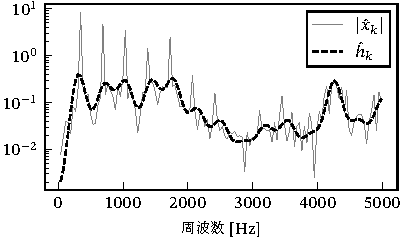
\includegraphics{figures/frequency_domain.pdf}
  \caption{「あ」の離散フーリエ変換.}
  \label{figure:frequency_domain}
\end{figure}

\cref{figure:frequency_domain}を見ると,\SI{350}{Hz}周辺に1つめのピークが現れている.これは\termdef{基本周波数}\index{きほんしゅうはすう@基本周波数}(fundamental frequency)と呼ばれる量で,人間が知覚する声の高さとかなりよく対応する.

\begin{note}
  人間が知覚する声の高さを\termdef{ピッチ}\index{ピッチ}(pitch)という.基本周波数とピッチはしばしば同一視されるが,厳密には定義からして異なる.詳しくは柏野\cite{kashino}など.
\end{note}

また,\cref{figure:frequency_domain}の破線部\(\hat{h}_k\)は,基本周波数に起因する細かな変動を\(\abs{\hat{x}_k}\)から除いた曲線である.
この曲線は\termdef{スペクトル包絡}\index{すぺくとるほうらく@スペクトル包絡}(spectral envelope)といい,音声の音色とよく対応する.
つまり,離散フーリエ変換を使うことで,音声が持つ基本周波数(≒声の高さ)由来の性質と,スペクトル包絡(≒音色)由来の性質を分離して解析できる.

\subsection{エイリアシング}

さきほど「\(\sqrt{N}\midx{w}{k}{n}=\napr^{2\krez\iuni kn/N}\)は周波数\(k/N\)の波である」と述べたが,この表現には少し語弊がある.

周波数\(f\)\,\si{Hz}の波\(\napr^{2\krez\iuni ft}\)について,瞬時値を1秒あたり\(f_{\symrm{s}}\)回記録すると数列\(\seq{\napr^{2\krez\iuni fn/f_{\symrm{s}}}}_{n\in\numset{Z}}\)ができる.
一方,周波数(\(f-f_{\symrm{s}}\))\,\si{Hz}の波\(\napr^{2\krez\iuni(f-f_{\symrm{s}})t}\)について同じ方法で数列を作ると,
その一般項は\(\napr^{2\krez\iuni(f-f_{\symrm{s}})n/f_{\symrm{s}}}=\napr^{2\krez\iuni fn/f_{\symrm{s}}}(\napr^{-2\krez\iuni})^n=\napr^{2\krez\iuni fn/f_{\symrm{s}}}\)となる.
つまり,周波数が\(f\)\,\si{Hz}でも(\(f-f_{\symrm{s}}\))\,\si{Hz}でも,できる数列は変わらない.

\begin{note}
  波が普通と逆向きに進むのを,周波数に負号をつけて表すことがある.特に,複素指数関数\(\napr^{-2\krez\iuni ft}\)(\(f>0\))は周波数\(-f\)の波とみなされる.
\end{note}

言い換えると,周波数が\(f_{\symrm{s}}\)だけ異なる波は数列から区別できない.\cref{figure:aliasing}は\(f_{\symrm{s}}=\SI{2.5}{Hz}\)のとき,
周波数\SI{2}{Hz}の波\(\sin(4\krez t)\)と\SI{-0.5}{Hz}の波\(\sin(-\krez t)\)が,時刻\(n/f_{\symrm{s}}\)秒(\(n\in\numset{Z}\))では同じ瞬時値を持つことを示している.

\begin{figure}[htbp]
  \centering
  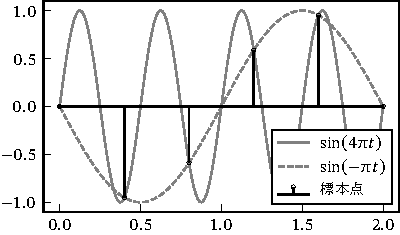
\includegraphics{figures/aliasing.pdf}
  \caption{エイリアシングの様子.}
  \label{figure:aliasing}
\end{figure}

一般に,連続信号から離散信号を得る操作を\termdef{標本化}\index{ひょうほんか@標本化}\index{サンプリング|see{標本化}}(sampling)といい,標本化によって信号が区別できなくなる現象を\termdef{エイリアシング}\index{エイリアシング}(aliasing)という.
また,\(f_{\symrm{s}}\)を\termdef{標本化周波数}\index{ひょうほんかしゅうはすう@標本化周波数}(sampling frequency)という.

\cref{figure:aliasing}の場合,標本化後の信号は周波数の絶対値が小さい(つまり低周波である)\SI{-0.5}{Hz}の波を表すと考えるほうが自然だろう.
周波数\(f\)の波を標本化すると,\(f\)より低周波の波と区別できなくなるのは\(\abs{f}\geq f_{\symrm{s}}/2\)のときである.\(f_{\symrm{s}}/2\)のことを\termdef{ナイキスト周波数}\index{ないきすとしゅうはすう@ナイキスト周波数}(Nyquist frequency)という.

話を離散フーリエ変換に戻すと,\(\sqrt{N}\midx{w}{k}{n}=\napr^{2\krez\iuni kn/N}\)は\(f=k\)の波が\(f_{\symrm{s}}=N\)で標本化されたものとみなせる.
そのため,\(k\geq N/2\)のとき\(\sqrt{N}\midx{w}{k}{n}\)は周波数\(k/N\)の波ではなく,周波数\((k-N)/N\)の波を表すとみなすのが普通である.

\subsection{曲線あてはめとDFT}

離散フーリエ変換は曲線あてはめの観点からも理解できる.周期\(2\krez\)の関数\(f\)を,複素指数関数の線型結合
\[
  f(\vect{c};t) = c_0\phi_0(t)+\dots+c_{K-1}\phi_{K-1}(t)\quad(\phi_k(t)=\exp(\iuni kt))
\]
で近似しよう.標本化周波数\(N\)で\(f\)を標本化すると,離散信号\(x[n]=f(t_n)\)(\(t_n=2\krez n/N\))が得られる\footnote{信号処理では慣習的に,整数値などの離散的な引数を大かっこで書く.}.

\(N\)個の標本\(f(t_n)=x[n]\)(\(0\leq n<N\))を用いて\(f\)を\(f(\vect{c};t)\)にあてはめる場合,\(K\)を\(N\)より大きくとると,\(\phi_0,\dots,\phi_{K-1}\)の中に標本化後は区別できなくなる組が現れてしまう(たとえば\(\phi_0\)と\(\phi_N\)).そこで\(K=N\)とし,残差平方和
\[
  \epsilon(\vect{c}) = \sum_{n=0}^{N-1}\abs{x[n]-f(\vect{c};t_n)}^2\quad(t_n=2\krez n/N)
\]
の値を最も小さくする\(\vect{c}\in\numset{C}^N\)を求める.それには正規方程式\(\htrps{\mat{\Phi}}\mat{\Phi}\vect{c}=\htrps{\mat{\Phi}}\vect{x}\)を解けばよい.ただし\(\vect{x}=\trps{\rowvect{x[0] & \cdots & x[N-1]}}\)かつ
\[
  \mat{\Phi} = \trps{\matfence{\phi_{i-1}(t_{j-1})}}
  = \matrice*{\napr^{\iuni\cdot 0(2\krez\cdot 0/N)} & \cdots & \napr^{\iuni(N-1)(2\krez\cdot 0/N)} \\ \vdots & \ddots & \vdots \\ \napr^{\iuni\cdot 0(2\krez(N-1)/N)} & \cdots & \napr^{\iuni(N-1)(2\krez(N-1)/N)}}
\]
である.ところが,\(\mat{\Phi}\)は\cref{proposition:dft_onb}の正規直交基底を用いて\(\sqrt{N}\mat{W}\)(\(\mat{W}=\rowvect{\vect{w}_0 & \cdots & \vect{w}_{N-1}}\))と書けるので\(\htrps{\mat{\Phi}}\mat{\Phi}=N\htrps{\mat{W}}\mat{W}=N\imat\)である.
つまり,正規方程式は初めから解かれているも同然であり,解は\(\vect{c}=(1/N)\htrps{\mat{\Phi}}\vect{x}=(1/\sqrt{N})\htrps{\mat{W}}\vect{x}=(1/\sqrt{N})\dft{N}\vect{x}\)である.

まとめると,区間\(\ccival{0}{2\krez}\)を\(N\)等分した左端における\(f\)の値を標本とし,関数\(f(\vect{c};t)=\sum_{k=0}^{N-1}c_k\napr^{\iuni kt}\)で\(f\)を最もよく近似しようとすると,係数\(\vect{c}\)は\(\dft{N}\vect{x}\)の定数倍になる.
また,各\(\phi_0,\dots,\phi_{N-1}\)を\(\sqrt{N}\)で割っておけば\(\vect{c}\)は完全に\(\dft{N}\vect{x}\)と等しくなる.

\begin{note}
  標本化周波数\(N\)の値を大きくすれば,より多くの標本,より高周波の複素指数関数を近似に使える.そこで\(N\to\infty\)の極限をとってみよう.エイリアシングを考慮すると,形式的には
  \begin{gather*}
    f(\vect{c};t) = \sum_{k=-N/2}^{N/2-1}c_k\napr^{\iuni kt}
    \to \sum_{k=-\infty}^\infty c_k\napr^{\iuni kt}, \\
    c_k = \frac{1}{N}\sum_{n=0}^{N-1}f(t_n)\napr^{-\iuni kt_n}
    = \frac{1}{2\krez}\sum_{n=0}^{N-1}f(t_n)\napr^{-\iuni kt_n}\frac{2\krez}{N}
    \to \frac{1}{2\krez}\int_0^{2\krez}f(t)\napr^{-\iuni kt}\intd{t}
  \end{gather*}
  となる.無限に高い周波数まで近似に含めたのだから,\(c_k=(1/(2\krez))\int_0^{2\krez}f(t)\napr^{-\iuni kt}\intd{t}\)のとき\(f(t)=\sum c_k\napr^{\iuni kt}\)が成り立つと期待するのは自然だろう.
  詳しくは\cref{xr-chapter:hilbert_space}で説明するが,式\(f(t)=\sum c_k\napr^{\iuni kt}\)を\(f\)のフーリエ級数展開\index{ふーりえきゅうすうてんかい@フーリエ級数展開}といい,\(f\)に適切な仮定を課せば実際に等式が成り立つことを証明できる.
\end{note}

\subsection{巡回畳み込み}

以下に\cref{equation:idft}を再掲する.
\[
  x_n = \frac{1}{\sqrt{N}}\sum_{k=0}^{N-1}\hat{x}_k\napr^{2\krez\iuni kn/N}
\]

\cref{equation:idft}は本来,\(\vect{x}=\trps{\rowvect{x_0 & \cdots & x_{N-1}}}\)を\(\dft{N}\vect{x}\)によって表す式である.
しかし,それをひとまず忘れて\(n\)に任意の整数を代入すれば,\(\vect{x}\)を周期\(N\)の数列\(\seq{x[n]}_{n\in\numset{Z}}\)へと拡張できる.
そこで,周期\(N\)の複素数列\(x=\seq{x[n]}_{n\in\numset{Z}}\)に対して\(\hat{x}=\dft{N}x\)を次のように定義する.

\begin{definition}{}{cycle_dft}\index{りさんふーりえへんかん@離散フーリエ変換!しゅうきすうれつ@周期数列}\indexsymbol{\(\cycles{\numset{C}}{N}\)}\index{FZN@\(\dft{N}\)}
  \(N\)を周期に持つ複素数列の全体集合を\(\cycles{\numset{C}}{N}\)と書く.線型写像\(\dft{N}\colon\cycles{\numset{C}}{N}\to\cycles{\numset{C}}{N}\)を次式で定義する.
  \[
    (\dft{N}x)[k] =  \frac{1}{\sqrt{N}}\sum_{n=0}^{N-1}x[n]\napr^{-2\krez\iuni kn/N}\quad(k\in\numset{Z})
  \]
\end{definition}

明らかに\(\cycles{\numset{C}}{N}\)は数列空間の部分空間である.\(\cycles{\numset{C}}{N}\)上の\termdef{ラグ作用素}\index{らぐさようそ@ラグ作用素}(lag operator)\(\lagop\)を\(\lagop x=\seq{x[n-1]}\)で定義し,数列\(\delta\in\cycles{\numset{C}}{N}\)を
\[
  \delta[n] = \begin{cases}1 & \text{(\(n\)は\(N\)で割り切れる)},\\ 0 & \text{(otherwise)}\end{cases}
\]
と定める.

\begin{proposition}{}{}
  集合\(\basis{D}=\Set{\lagop^m\delta\given 0\leq m<N}\)は\(\cycles{\numset{C}}{N}\)の基底である.ただし\(\lagop^0\delta=\delta\)とする.
\end{proposition}

\begin{proof}
  \(x\in\cycles{\numset{C}}{N}\),\(m,n\in\Set{0,\dots,N-1}\)を任意にとる.\(\abs{n-m}<N\)なので,\(n-m\)が\(N\)で割り切れるのは\(n-m=0\)のときだけである.
  よって\(x[m](\lagop^m\delta)[n]=x[m]\delta[n-m]=x[n]\kdelta{m}{n}\)であり,\(m\)に関して和をとると
  \[
    \sum_{m=0}^{N-1}x[m](\lagop^m\delta)[n] = x[n]\sum_{m=0}^{N-1}\kdelta{m}{n}
    = x[n]
  \]
  となる.よって\(x=\sum_{m=0}^{N-1}x[m]\lagop^m\delta\)なので,\(\basis{D}\)は\(\cycles{\numset{C}}{N}\)の基底である.
\end{proof}

\begin{figure}[htbp]
  \centering
  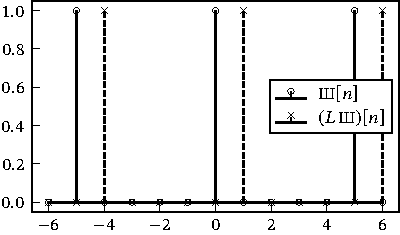
\includegraphics{figures/comb.pdf}
  \caption{\(N=5\)のときの\(\delta\)と\(\lagop\delta\)の様子.}
\end{figure}

\begin{proposition}{}{dft_shift_theorem}
  任意の\(x\in\cycles{\numset{C}}{N}\)に対して\((\dft{N}\lagop x)[k]=\zeta^{-k}\hat{x}[k]\)である.
\end{proposition}

\begin{proof}
  \(\sum\)の添字\(n\)を\(m=n+1\)に置き換えると
  \[
    \zeta^{-k}\hat{x}[k] = \frac{1}{\sqrt{N}}\sum_{n=0}^{N-1}x[n]\napr^{-2\krez\iuni k(n+1)/N}
    = \frac{1}{\sqrt{N}}\sum_{m=1}^Nx[m-1]\napr^{-2\krez\iuni km/N}
  \]
  となる.右辺は周期数列の1周期に渡る和だから,\(\sum_{m=1}^N\)を\(\sum_{m=0}^{N-1}\)に変えても値は変わらない.よって\(\zeta^{-k}\hat{x}[k]=(\dft{N}\lagop x)[k]\)である.
\end{proof}

\cref{proposition:dft_shift_theorem}を使うと,数列の積\(x\cdot y=\seq{x[n]y[n]}\)と離散フーリエ変換の間にある関係を示せる.積は\(\dft{N}\)で,次の2項演算へと写される.

\begin{definition}{巡回畳み込み}{}\index{じゅんかいたたみこみ@巡回畳み込み}\index{たたみこみ@畳み込み!じゅんかい@巡回}\indexsymbol{\(x\circconv y\)}
  \(x,y\in\cycles{\numset{C}}{N}\)とする.次式で定義される\(x\circconv y\in\cycles{\numset{C}}{N}\)を\(x\)と\(y\)の\termdef{巡回畳み込み}(circular convolution)という.
  \[
    (x\circconv y)[n] = \sum_{m=0}^{N-1}x[m]y[n-m]\quad(n\in\numset{Z})
  \]
\end{definition}

\(y[n-m]=(\lagop^my)[n]\)だから,巡回畳み込みは次のように表せる.
\begin{equation}
  \label{equation:discrete_impulse_response}
  x\circconv y = \sum_{m=0}^{N-1}x[m]\lagop^my
  = \pqty*{\sum_{m=0}^{N-1}x[m]\lagop^m}y
\end{equation}

\begin{proposition}{}{dft_convolution_theorem}
  任意の\(x,y\in\cycles{\numset{C}}{N}\)に対して次式が成立する.
  \[
    \dft{N}(x\circconv y) = \sqrt{N}\hat{x}\cdot\hat{y},
    \quad\dft{N}(x\cdot y) = \frac{1}{\sqrt{N}}\hat{x}\circconv\hat{y}
  \]
\end{proposition}

\begin{proof}
  1つめのみ示す.\(z=x\circconv y\)とすると,\cref{equation:discrete_impulse_response}から
  \[
    \hat{z} = \dft{N}\pqty*{\sum_{m=0}^{N-1}x[m]\lagop^my}
    = \sum_{m=0}^{N-1}x[m]\dft{N}\lagop^my
  \]
  であり,\cref{proposition:dft_shift_theorem}より\((\dft{N}\lagop^my)[k]=(\zeta^{-k})^m\hat{y}[k]\)なので
  \[
    \hat{z}[k] = \sum_{m=0}^{N-1}x[m](\zeta^{-km}\hat{y}[k])
    = \pqty*{\sum_{m=0}^{N-1}x[m]\zeta^{-km}}\hat{y}[k]
    = \sqrt{N}\hat{x}[k]\hat{y}[k]
  \]
  となる.よって\(\hat{z}=\sqrt{N}\hat{x}\cdot\hat{y}\)である.
\end{proof}

\begin{corollary}{}{circular_convolution_properties}
  任意の\(x,y,z\in\cycles{\numset{C}}{N}\)に対して,以下の式が成立する.
  \begin{enumerate}
    \item \(x\circconv y=y\circconv x\)
    \item \((x\circconv y)\circconv z=x\circconv (y\circconv z)\)
    \item \(x\circconv(y+z)=(x\circconv y)+(x\circconv z)\)
  \end{enumerate}
\end{corollary}

\begin{proof}
  2つめのみ示す.\(\dft{N}(x\circconv (y\circconv z))=\sqrt{N}\hat{x}\cdot\dft{N}(y\circconv z)=N\hat{x}\cdot(\hat{y}\cdot\hat{z})\)より
  \(x\circconv(y\circconv z)=N\dft{N}^{-1}(\hat{x}\cdot\hat{y}\cdot\hat{z})\)であり,同じ計算によって\((x\circconv y)\circconv z=N\dft{N}^{-1}(\hat{x}\cdot\hat{y}\cdot\hat{z})\)も確かめられる.
\end{proof}

\(\cycles{\numset{C}}{N}\)で得られた結果を\(\numset{C}^N\)で使える形に書き換えよう.
\(\numset{C}^N\)の標準基底を\(\Set{\vect{e}_1,\dots,\vect{e}_N}\)とおく.各\(x\in\cycles{\numset{C}}{N}\),\(\vect{x}=\trps{\rowvect{x[0] & \cdots & x[N-1]}}\)に対して
\[
  \trps{\vect{x}}\matrice{\vect{e}_N & \vect{e}_1 & \cdots & \vect{e}_{N-1}}
  = \matrice{x[-1] & x[0] & \cdots & x[N-2]}
\]
なので,基底\(\basis{D}\)に関する\(\lagop\)の表現行列\(\mat{L}\)は\(\mat{L}=\trps{\rowvect{\vect{e}_N & \vect{e}_1 & \cdots & \vect{e}_{N-1}}}=\smallmatrice{ & 1 \\ \imat_{N-1} & }\)と書ける.
同様に計算すれば,\(0<m<N\)のとき\(\lagop^m\)の表現行列は\(\mat{L}^m=\smallmatrice{ & \imat_m \\ \imat_{N-m} & }\)であることも分かる.

\(h\in\cycles{\numset{C}}{N}\)を任意にとり,\(\cycles{\numset{C}}{N}\)上の線型写像\(H\)を\(H(x)=h\circconv x\)で定義する.
\cref{equation:discrete_impulse_response}から\(H=\sum_{m=0}^{N-1}h_m\lagop^m\)(\(h_m=h[m]\))なので,\(H\)の表現行列\(\mat{H}\)は
\[
  \mat{H} = h_0\imat+\sum_{m=1}^{N-1}h_m\matrice*{ & \imat_m \\ \imat_{N-m} & }
  = \matrice*{h_0 & h_{N-1} & \cdots & h_2 & h_1 \\ h_1 & h_0 & h_{N-1} & \ddots & h_2 \\ h_2 & h_1 & \ddots & \ddots & \vdots \\ \vdots & \ddots & \ddots & h_0 & h_{N-1} \\ h_{N-1} &\cdots & h_2 & h_1 & h_0}
\]
である.この形の行列を\termdef{巡回行列}\index{じゅんかいぎょうれつ@巡回行列}\index{ぎょうれつ@行列!じゅんかい@巡回\texttwoemdash}(circulant matrix)という.

基底\(\basis{D}\)に関する\(\dft{N}\)の表現行列を\(\htrps{\mat{W}}\)とおく.\(\htrps{\mat{W}}\)は\(\numset{C}^N\)上で定義した\(\dft{N}\)の,標準基底に関する表現行列でもある.

\begin{corollary}{}{dft_convolution_matrix}
  巡回行列は離散フーリエ変換で対角化される.すなわち,任意の\(N\)次巡回行列\(\mat{H}\)について\(\htrps{\mat{W}}\mat{H}\mat{W}\)は対角行列である.
\end{corollary}

\begin{proof}
  \(\mat{H}\)の第1列を\(\trps{\rowvect{h_0 & \cdots & h_{N-1}}}\)とおき,\(h[n]=h_n\)(\(0\leq n<N\))となるように\(\cycles{\numset{C}}{N}\)の元\(h\)を定める.
  \(\cycles{\numset{C}}{N}\)上の線型写像\(H\)を\(H(x)=h\circconv x\)で定義すると,\cref{proposition:dft_convolution_theorem}より\((\dft{N}H\dft{N}^{-1})x=\dft{N}(h\circconv\dft{N}^{-1}x)=\hat{h}\cdot x\)となる.よって,\(\dft{N}H\dft{N}^{-1}\)の表現行列は\(\diag(\hat{h}[0],\dots,\hat{h}[N-1])\)である.

  一方,\(H\)の表現行列は\(\mat{H}\)だから\(\dft{N}H\dft{N}^{-1}\)の表現行列は\(\htrps{\mat{W}}\mat{H}\mat{W}\)でもある.
  したがって\(\htrps{\mat{W}}\mat{H}\mat{W}\)は対角行列である.
\end{proof}

\begin{example}
  \label{example:cyclic_filter}
  \(N=32\)とし,\(\cycles{\numset{C}}{N}\)の元\(h\)を\(h[n]=1/3\)(\(0\leq n<3\)),\(h[n]=0\)(\(3\leq n<N\))で定義する.このとき
  \[
    (h\circconv x)[n] = \sum_{m=0}^{N-1}h[m]x[n-m]
    = \frac{x[n]+x[n-1]+x[n-2]}{3}
  \]
  だから,\((h\circconv x)[n]\)は時刻\(n,n-1,n-2\)における\(x\)の値の平均である.

  平均をとると細かい変動が均されるので,高周波の成分は減るだろう.実際\(\abs{\hat{h}[k]}=(1/3)\abs{\zeta^{-k\cdot 0}+\zeta^{-k\cdot 1}+\zeta^{-k\cdot 2}}\)のグラフは\cref{figure:filter_characteristics}のようになり,\(\dft{N}(h\circconv x)=\hat{h}\cdot\hat{x}\)だから\(h\)を畳み込むと高周波は削られる.
\end{example}

\begin{figure}[htbp]
  \centering
  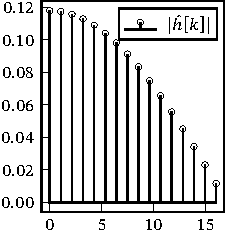
\includegraphics{figures/filter_characteristics.pdf}
  \caption{\(\abs{\hat{h}[k]}\)の様子.エイリアシングを考慮し\(0\leq k\leq 16\)で図示した.}
  \label{figure:filter_characteristics}
\end{figure}

\subsection{多次元DFT}

\begin{definition}{多次元離散フーリエ変換}{multidimensional_discrete_fourier_transform}\index{りさんふーりえへんかん@離散フーリエ変換!たじげん@多次元}\index{FZdn@\(\dft[d]{\vect{n}}\)}
  \(\vect{n}=\trps{\rowvect{N_1 & \cdots & N_d}}\)を自然数の組とし,\(\Omega=\Set{\trps{\rowvect{u_1 & \cdots & u_d}}\given\text{\(u_i\in\numset{Z}\),\(0\leq u_i<N_i\)(\(1\leq i\leq d\))}}\),\(\mat{N}=\diag(N_1,\dots,N_d)\)とおく.
  関数\(x\in\mapset{\Omega}{\numset{C}}\)に対して,関数
  \[
    \hat{x}[\vect{k}] = \frac{1}{\sqrt{\det\mat{N}}}\sum_{\vect{r}\in\Omega}x[\vect{r}]\napr^{-2\krez\iuni\trps{\vect{k}}\mat{N}^{-1}\vect{r}}\quad(\vect{k}\in\Omega)
  \]
  を対応づける線型写像\(\dft[d]{\vect{n}}\colon\mapset{\Omega}{\numset{C}}\to\mapset{\Omega}{\numset{C}}\)を\termdef{\(d\)次元離散フーリエ変換}という.
\end{definition}

特に\(d=2\)のとき(\(\sum\)の添字\(r_i\)は集合\(\Set{0,\dots,N_i-1}\)上を動くとして)
\begin{align*}
  \hat{x}[k_1,k_2] &= \frac{1}{\sqrt{N_1N_2}}\sum_{r_2}\sum_{r_1}x[r_1,r_2]\napr^{-2\krez\iuni(k_1r_1/N_1+k_2r_2/N_2)} \\
  &= \frac{1}{\sqrt{N_2}}\sum_{r_2}\pqty*{\frac{1}{\sqrt{N_1}}\sum_{r_1}x[r_1,r_2]\napr^{-2\krez\iuni k_1r_1/N_1}}\napr^{-2\krez\iuni k_2r_2/N_2}
\end{align*}
であり,右辺は\(x[r_1,r_2]\)を各変数に関して離散フーリエ変換した形になっている.
より一般に,\(x[r_1,\dots,r_d]\)の\(d\)次元離散フーリエ変換は,\(x[r_1,\dots,r_d]\)を各変数に関して離散フーリエ変換したものと一致する.

次の命題は,一般の次元で離散フーリエ変換が分析作用素であることを示している.
ただし,\(\mapset{\Omega}{\numset{C}}\)の内積は\(\innerp{x}{y}=\sum_{\vect{r}\in\Omega}x[\vect{r}]\conj*{y[\vect{r}]}\)で定義する.

\begin{proposition}{}{ddimdft_onb}
  \(w_{\vect{k}}[\vect{r}]=(\det\mat{N})^{-1/2}\exp(2\krez\iuni\trps{\vect{k}}\mat{N}^{-1}\vect{r})\)とする.このとき,集合\(\Set{w_{\vect{k}}\given\vect{k}\in\Omega}\)は\(\mapset{\Omega}{\numset{C}}\)の正規直交基底である.
\end{proposition}

\begin{proof}
  \(\Omega\)から2元\(\vect{i}=\trps{\rowvect{i_1 & \cdots & i_d}}\),\(\vect{j}=\trps{\rowvect{j_1 & \cdots & j_d}}\)を任意にとる.
  \(w_{\vect{i}}[\vect{r}]\conj*{w_{\!\vect{j}}[\vect{r}]}=(1/\det\mat{N})\exp(2\krez\iuni\trps{(\vect{i}-\vect{j})}\mat{N}^{-1}\vect{r})\)(\(\vect{r}=\trps{\rowvect{r_1 & \cdots & r_d}}\))は
  \[
    w_{\vect{i}}[\vect{r}]\conj*{w_{\!\vect{j}}[\vect{r}]} = \frac{1}{N_1\dotsm N_d}\exp\pqty*{\sum_{k=1}^d\frac{2\krez\iuni(i_k-j_k)r_k}{N_k}}
    = \prod_{k=1}^d\frac{\napr^{2\krez\iuni(i_k-j_k)r_k/N_k}}{N_k}
  \]
  と計算できるので,\(\zeta_k=\napr^{2\krez\iuni/N_k}\)とおくと
  \[
    \sum_{\vect{r}\in\Omega}w_{\vect{i}}[\vect{r}]\conj*{w_{\!\vect{j}}[\vect{r}]} = \sum_{r_1}\dotsm\sum_{r_d}\prod_{k=1}^d\frac{\zeta_k^{(i_k-j_k)r_k}}{N_k}
    = \prod_{k=1}^d\sum_{r_k}\frac{\zeta_k^{(i_k-j_k)r_k}}{N_k}
  \]
  である.よって\cref{proposition:dft_onb}より\(\innerp{w_{\vect{i}}}{w_{\!\vect{j}}}=\prod_{k=1}^d\kdelta{i_k}{j_k}=\kdelta{\vect{i}}{\vect{j}}\)である.
\end{proof}

\cref{proposition:ddimdft_onb}と\(\hat{x}[\vect{k}]=\innerp{x}{w_{\vect{k}}}\)より,\(\dft[d]{N}\)の逆変換は
\[
  x[\vect{r}] = \sum_{\vect{k}\in\Omega}\innerp{x}{w_{\vect{k}}}w_{\vect{k}}
  = \frac{1}{\sqrt{\det\mat{N}}}\sum_{\vect{k}\in\Omega}\hat{x}[\vect{k}]\napr^{2\krez\iuni\trps{\vect{k}}\mat{N}^{-1}\vect{r}}
\]
である.

2次元離散フーリエ変換は画像処理に応用されている.

\begin{figure}[htbp]
  \begin{minipage}{\linewidth/2}
    \centering
    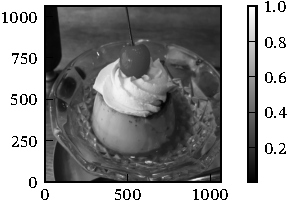
\includegraphics{figures/pudding.pdf}
  \end{minipage}%
  \begin{minipage}{\linewidth/2}
    \centering
    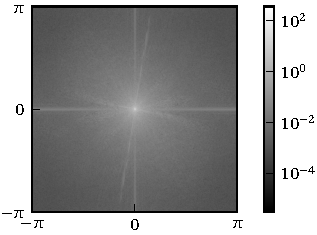
\includegraphics{figures/pudding_dft.pdf}
  \end{minipage}
  \caption{画像とその2次元DFT.}
  \label{figure:pudding_dft}
\end{figure}

\cref{figure:pudding_dft}は,画像を離散信号\(s=\seq{s[x,y]}\)とみなし\(\abs{\hat{s}[u,v]}\)を計算した様子である.
ただし\(\vect{n}\)は,この画像が\(1024\times 1024\)の画素からなるので\(\vect{n}=\smallmatrice{N \\ N}\)(\(N=1024\))である.

\(\hat{s}[u,v]\)は\(x\)と\(y\)に関して\(s[x,y]\)を離散フーリエ変換したものだから,\(u\geq N/2\)か\(v\geq N/2\)のときはエイリアシングが起きている.
つまり,低周波にもかかわらず原点から遠いところにプロットされている領域がある.
低周波ほど原点の近くにプロットするには,\(u\geq N/2\)のとき\(u\)を\(u-N\)に,\(v\geq N/2\)のとき\(v\)を\(v-N\)に置き換えてプロットしなおせばよい.
そのとき\cref{figure:pudding_dft}は次のように変化する.

\begin{figure}[htbp]
  \centering
  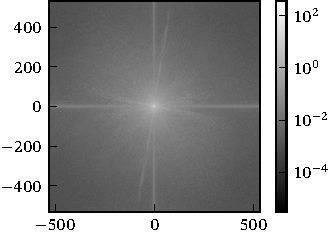
\includegraphics{figures/pudding_shift.pdf}
  \caption{エイリアシングを補正した2次元DFTの様子.}
  \label{figure:pudding_shift}
\end{figure}

\begin{figure}[htbp]
  \begin{minipage}{\linewidth/2}
    \centering
    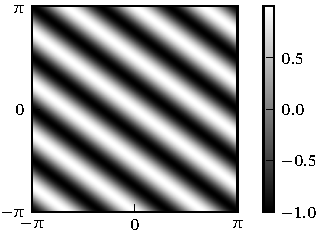
\includegraphics{figures/2dcos.pdf}
    \end{minipage}%
  \begin{minipage}{\linewidth/2}
    \centering
    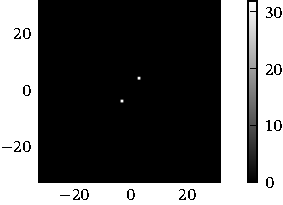
\includegraphics{figures/2dcos_dft.pdf}
  \end{minipage}
  \caption{\(\cos(3x+4y)\)(\(x,y\in\Set{2\krez(k-32)/64\given\text{\(k\in\numset{Z}\),\(0\leq k<64\)}}\))のグラフと2次元離散フーリエ変換.}
\end{figure}

\section{多重解像度解析}

\section{補遺}

\subsection{スペクトル定理の証明}
\label{subsection:proof_of_the_spectral_theorem}

\cref{theorem:spectral_theorem}を証明する前に,次の定理を示そう.

\begin{theorem}{シューア分解}{schur_decomposition}\index{しゅーあぶんかい@シューア分解}\index{うえさんかくぎょうれつ@上三角行列}\index{ぎょうれつ@行列!うえさんかく@上三角\texttwoemdash}
  任意の複素正方行列はユニタリ行列で上三角化できる.すなわち,任意の\(n\)次複素正方行列\(\mat{A}\)に対し,
  \(n\)次ユニタリ行列\(\mat{U}\)が存在して,\(\mat{A}'=\htrps{\mat{U}}\mat{A}\mat{U}\)は上三角行列\footnotemark になる.
  式\(\mat{A}=\mat{U}\mat{A}'\htrps{\mat{U}}\)を\(\mat{A}\)の\termdef{シューア分解}(Schur decomposition)という.
\end{theorem}

\begin{proof}
  \footnotetext{\(\midx{a}{i}{j}=0\)(\(i>j\))である正方行列\(\matfence{\midx{a}{i}{j}}\)を\termdef{上三角行列}(upper triangular matrix)という.}
  \(n\)に関する帰納法で示す.\(\vect{u}_1\)を\(\mat{A}\)のある固有値\(\lambda\)に属する,ノルム1の固有ベクトルとする.
  また,集合\(\Set{\vect{u}_2,\dots,\vect{u}_n}\)を\(\pcomp{(\spannedby\Set{\vect{u}_1})}\)の正規直交基底とする.
  このとき,集合\(\Set{\vect{u}_1,\dots,\vect{u}_n}\)は\(\numset{C}^n\)の正規直交基底だから,\(\vect{U}=\rowvect{\vect{u}_1 & \cdots & \vect{u}_n}\)はユニタリ行列である.

  \(\numset{C}^n\)の元\(\vect{e}_1\)を\(\vect{e}_1=\trps{\rowvect{1 & 0 & \cdots & 0}}\)で定めると,\(\htrps{\mat{U}}\mat{A}\vect{u}_1=\htrps{\mat{U}}(\lambda\vect{u}_1)=\lambda\vect{e}_1\)なので
  \(\htrps{\mat{U}}\mat{A}\mat{U}=\rowvect{\lambda\vect{e}_1 & \htrps{\mat{U}}\mat{A}\vect{u}_2 & \cdots & \htrps{\mat{U}}\mat{A}\vect{u}_n}\)である.
  右辺を\(\smallmatrice{\lambda & \trps{\vect{b}} \\ & \mat{C}}\)とおく(\(\mat{C}\)は\(n-1\)次正方行列,\(\vect{b}\in\numset{C}^{n-1}\)).
  帰納法の仮定から\(\mat{C}\)はシューア分解できる.\(\mat{C}=\mat{V}\mat{C}'\htrps{\mat{V}}\)をシューア分解とし,\(n\)次ユニタリ行列\(\mat{W}\)を\(\mat{W}=\smallmatrice{1 & \\ & \mat{V}}\)で定義する.このとき
  \[
    \matrice*{\lambda & \trps{\vect{b}} \\ & \mat{C}} = \matrice*{\lambda & \trps{\vect{b}} \\ & \mat{V}\mat{C}'\htrps{\mat{V}}}
    = \matrice*{1 & \\ & \mat{V}}\matrice*{\lambda & \trps{\vect{b}}\mat{V} \\ & \mat{C}'}\matrice*{1 & \\ & \htrps{\mat{V}}}
  \]
  なので,\(\mat{A}'=\smallmatrice{\lambda & \trps{\vect{b}}\mat{V} \\ & \mat{C}'}\)とおくと\(\htrps{\mat{U}}\mat{A}\mat{U}=\mat{W}\mat{A}'\htrps{\mat{W}}\)である.
  よって,\(\mat{U}\mat{W}\)をあらためて\(\mat{U}\)とすれば\(\mat{A}=\mat{U}\mat{A}'\htrps{\mat{U}}\)で,\(\mat{A}'\)は上三角行列だから,これは\(\mat{A}\)のシューア分解になっている.
\end{proof}

\cref{theorem:schur_decomposition}を利用すると,\cref{theorem:spectral_theorem}は次のようにして示せる.

\begin{proof}[スペクトル定理の証明]
  ユニタリ行列で対角化できれば正規行列であることはすぐ分かる.
  \(\mat{A}\)を\(n\)次正規行列とする.\(\mat{A}\)のシューア分解を\(\mat{A}=\mat{U}\mat{B}\htrps{\mat{U}}\)とおくと,
  \(\htrps{\mat{A}}\mat{A}-\mat{A}\htrps{\mat{A}}=\mat{U}(\htrps{\mat{B}}\mat{B}-\mat{B}\htrps{\mat{B}})\htrps{\mat{U}}=\zmat\)より\(\mat{B}\)も正規行列である.

  \(\mat{B}=\matfence{\midx{b}{i}{j}}\)とおく.\(\htrps{\mat{B}}=\matfence{\midx{\conj{b}}{j}{i}}\),(\(i>j\implies\midx{b}{i}{j}=0\))なので,\(\htrps{\mat{B}}\mat{B}=\mat{B}\htrps{\mat{B}}\)の\(d\)行\(d\)列にある成分を比較すれば
  \[
    \sum_{i=1}^n\midx{\conj{b}}{i}{d}\midx{b}{i}{d} = \sum_{j=1}^n\midx{b}{d}{j}\midx{\conj{b}}{d}{j},
    \quad\sum_{i=1}^d\abs{\midx{b}{i}{d}}^2 = \sum_{j=d}^n\abs{\midx{b}{d}{j}}^2
  \]
  が分かる.\(d=1\)とすると,\(\abs{\midx{b}{1}{1}}^2=\sum_{j=1}^n\abs{\midx{b}{1}{j}}^2\)より\(\midx{b}{1}{2}=\dots=\midx{b}{1}{n}=0\)である.
  次に\(d=2\)とすると,\(\abs{\midx{b}{1}{2}}^2+\abs{\midx{b}{2}{2}}^2=\abs{\midx{b}{2}{2}}^2=\sum_{j=2}^n\abs{\midx{b}{2}{j}}^2\)より\(\midx{b}{2}{3}=\dots=\midx{b}{2}{n}=0\)である.
  同様に\(d=n\)まで計算すれば(\(i<j\implies\midx{b}{i}{j}=0\))が分かる.\(\mat{B}\)は上三角行列だから,これは\(\mat{B}\)が対角行列であることを意味する.
  つまり,シューア分解\(\mat{A}=\mat{U}\mat{B}\htrps{\mat{U}}\)は\(\mat{A}\)のスペクトル分解になっている.
\end{proof}

\subsection{主成分分析}

最小2乗法のもう一つの応用例として,\termdef{主成分分析}\index{しゅせいぶんぶんせき@主成分分析}\index{PCA|see{主成分分析}}(principal component analysis; PCA)という手法を紹介する.

変数\(\vect{x}=\trps{\rowvect{x_1 & \cdots & x_p}}\)の観測値\(\vect{x}_1,\dots,\vect{x}_n\)を眺めても,\(\vect{x}\)が高次元\footnote{\(p\)の値が非常に大きいこと.}だとその特徴が分かりにくいことがある.
主成分分析の目的は,この問題を解決するために\(\vect{x}\)の特徴を保ったまま次元を減らすことである.

\begin{figure}[htbp]
  \begin{minipage}{\linewidth/2}
    \centering
    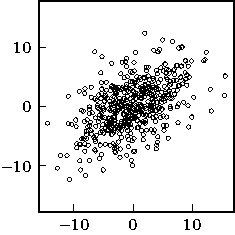
\includegraphics{figures/scatter.pdf}
  \end{minipage}%
  \begin{minipage}{\linewidth/2}
    \centering
    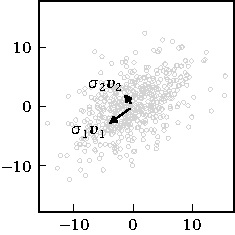
\includegraphics{figures/pca.pdf}
  \end{minipage}
\end{figure}

\section{演習問題}

\begin{enumerate}
  \item \cref{corollary:singular_value_decomposition}の証明を完成させよ.
  \item 任意の\(n\times p\)複素行列\(\mat{A}\),\(\vect{x}\in\numset{C}^p\),\(\vect{y}\in\numset{C}^n\)に対して,以下の式が成立することを示せ.
    \begin{gather*}
      \proj_{\nulsp\mat{A}}\vect{x} = (\imat-\pinv{\mat{A}}\mat{A})\vect{x},
      \quad\proj_{\pcomp{(\nulsp\mat{A})}}\vect{x} = \pinv{\mat{A}}\mat{A}\vect{x}, \\
      \proj_{\colsp\mat{A}}\vect{y} = \mat{A}\pinv{\mat{A}}\vect{y},
      \quad\proj_{\pcomp{(\colsp\mat{A})}}\vect{y} = (\imat-\mat{A}\pinv{\mat{A}})\vect{y}
    \end{gather*}
  \item \(n\)次複素正方行列\(\mat{A}\)に対して\(\exp\mat{A}\)を\(\exp\mat{A}=\sum_{k=0}^\infty\mat{A}^k/(k!)\)で定義する
    (この極限は各成分の極限で定義され,\(\exp\mat{A}\)を定義する級数は常に収束することが分かっている).
    \(\mat{A}\)が正規行列なら,そのスペクトル分解を\(\mat{A}=\mat{U}\diag(\lambda_1,\dots,\lambda_n)\htrps{\mat{U}}\)とすると
    \(\exp\mat{A}=\mat{U}\diag(\napr^{\lambda_1},\dots,\napr^{\lambda_n})\htrps{\mat{U}}\)であることを示せ.
  \item \(\dft{N}\vect{x}=\trps{\rowvect{\hat{x}_0 & \cdots & \hat{x}_{N-1}}}\)(\(\vect{x}=\trps{\rowvect{x_0 & \cdots & x_{N-1}}}\))のとき
  \begin{equation}
    \label{equation:dft_parseval}
    \sum_{k=0}^{N-1}\abs{\hat{x}_k}^2 = \sum_{n=0}^{N-1}\abs{x_n}^2
  \end{equation}
  であることを示せ.信号処理ではしばしば\cref{equation:dft_parseval}を\termdef{パーセヴァルの定理}\index{ぱーせばるのていり@パーセヴァルの定理}(Parseval's theorem),あるいは\termdef{プランシュレルの定理}\index{ぷらんしゅれるのていり@プランシュレルの定理}(Plancherel's theorem)と呼ぶ.  
\end{enumerate}

\end{document}
